% Options for packages loaded elsewhere
\PassOptionsToPackage{unicode}{hyperref}
\PassOptionsToPackage{hyphens}{url}
\PassOptionsToPackage{dvipsnames,svgnames,x11names}{xcolor}
%
\documentclass[
  12pt,
  a4paper,
  DIV=11,
  numbers=noendperiod]{scrartcl}

\usepackage{amsmath,amssymb}
\usepackage{iftex}
\ifPDFTeX
  \usepackage[T1]{fontenc}
  \usepackage[utf8]{inputenc}
  \usepackage{textcomp} % provide euro and other symbols
\else % if luatex or xetex
  \usepackage{unicode-math}
  \defaultfontfeatures{Scale=MatchLowercase}
  \defaultfontfeatures[\rmfamily]{Ligatures=TeX,Scale=1}
\fi
\usepackage{lmodern}
\ifPDFTeX\else  
    % xetex/luatex font selection
\fi
% Use upquote if available, for straight quotes in verbatim environments
\IfFileExists{upquote.sty}{\usepackage{upquote}}{}
\IfFileExists{microtype.sty}{% use microtype if available
  \usepackage[]{microtype}
  \UseMicrotypeSet[protrusion]{basicmath} % disable protrusion for tt fonts
}{}
\makeatletter
\@ifundefined{KOMAClassName}{% if non-KOMA class
  \IfFileExists{parskip.sty}{%
    \usepackage{parskip}
  }{% else
    \setlength{\parindent}{0pt}
    \setlength{\parskip}{6pt plus 2pt minus 1pt}}
}{% if KOMA class
  \KOMAoptions{parskip=half}}
\makeatother
\usepackage{xcolor}
\usepackage[margin=0.8in]{geometry}
\setlength{\emergencystretch}{3em} % prevent overfull lines
\setcounter{secnumdepth}{3}
% Make \paragraph and \subparagraph free-standing
\makeatletter
\ifx\paragraph\undefined\else
  \let\oldparagraph\paragraph
  \renewcommand{\paragraph}{
    \@ifstar
      \xxxParagraphStar
      \xxxParagraphNoStar
  }
  \newcommand{\xxxParagraphStar}[1]{\oldparagraph*{#1}\mbox{}}
  \newcommand{\xxxParagraphNoStar}[1]{\oldparagraph{#1}\mbox{}}
\fi
\ifx\subparagraph\undefined\else
  \let\oldsubparagraph\subparagraph
  \renewcommand{\subparagraph}{
    \@ifstar
      \xxxSubParagraphStar
      \xxxSubParagraphNoStar
  }
  \newcommand{\xxxSubParagraphStar}[1]{\oldsubparagraph*{#1}\mbox{}}
  \newcommand{\xxxSubParagraphNoStar}[1]{\oldsubparagraph{#1}\mbox{}}
\fi
\makeatother

\usepackage{color}
\usepackage{fancyvrb}
\newcommand{\VerbBar}{|}
\newcommand{\VERB}{\Verb[commandchars=\\\{\}]}
\DefineVerbatimEnvironment{Highlighting}{Verbatim}{commandchars=\\\{\}}
% Add ',fontsize=\small' for more characters per line
\usepackage{framed}
\definecolor{shadecolor}{RGB}{241,243,245}
\newenvironment{Shaded}{\begin{snugshade}}{\end{snugshade}}
\newcommand{\AlertTok}[1]{\textcolor[rgb]{0.68,0.00,0.00}{#1}}
\newcommand{\AnnotationTok}[1]{\textcolor[rgb]{0.37,0.37,0.37}{#1}}
\newcommand{\AttributeTok}[1]{\textcolor[rgb]{0.40,0.45,0.13}{#1}}
\newcommand{\BaseNTok}[1]{\textcolor[rgb]{0.68,0.00,0.00}{#1}}
\newcommand{\BuiltInTok}[1]{\textcolor[rgb]{0.00,0.23,0.31}{#1}}
\newcommand{\CharTok}[1]{\textcolor[rgb]{0.13,0.47,0.30}{#1}}
\newcommand{\CommentTok}[1]{\textcolor[rgb]{0.37,0.37,0.37}{#1}}
\newcommand{\CommentVarTok}[1]{\textcolor[rgb]{0.37,0.37,0.37}{\textit{#1}}}
\newcommand{\ConstantTok}[1]{\textcolor[rgb]{0.56,0.35,0.01}{#1}}
\newcommand{\ControlFlowTok}[1]{\textcolor[rgb]{0.00,0.23,0.31}{\textbf{#1}}}
\newcommand{\DataTypeTok}[1]{\textcolor[rgb]{0.68,0.00,0.00}{#1}}
\newcommand{\DecValTok}[1]{\textcolor[rgb]{0.68,0.00,0.00}{#1}}
\newcommand{\DocumentationTok}[1]{\textcolor[rgb]{0.37,0.37,0.37}{\textit{#1}}}
\newcommand{\ErrorTok}[1]{\textcolor[rgb]{0.68,0.00,0.00}{#1}}
\newcommand{\ExtensionTok}[1]{\textcolor[rgb]{0.00,0.23,0.31}{#1}}
\newcommand{\FloatTok}[1]{\textcolor[rgb]{0.68,0.00,0.00}{#1}}
\newcommand{\FunctionTok}[1]{\textcolor[rgb]{0.28,0.35,0.67}{#1}}
\newcommand{\ImportTok}[1]{\textcolor[rgb]{0.00,0.46,0.62}{#1}}
\newcommand{\InformationTok}[1]{\textcolor[rgb]{0.37,0.37,0.37}{#1}}
\newcommand{\KeywordTok}[1]{\textcolor[rgb]{0.00,0.23,0.31}{\textbf{#1}}}
\newcommand{\NormalTok}[1]{\textcolor[rgb]{0.00,0.23,0.31}{#1}}
\newcommand{\OperatorTok}[1]{\textcolor[rgb]{0.37,0.37,0.37}{#1}}
\newcommand{\OtherTok}[1]{\textcolor[rgb]{0.00,0.23,0.31}{#1}}
\newcommand{\PreprocessorTok}[1]{\textcolor[rgb]{0.68,0.00,0.00}{#1}}
\newcommand{\RegionMarkerTok}[1]{\textcolor[rgb]{0.00,0.23,0.31}{#1}}
\newcommand{\SpecialCharTok}[1]{\textcolor[rgb]{0.37,0.37,0.37}{#1}}
\newcommand{\SpecialStringTok}[1]{\textcolor[rgb]{0.13,0.47,0.30}{#1}}
\newcommand{\StringTok}[1]{\textcolor[rgb]{0.13,0.47,0.30}{#1}}
\newcommand{\VariableTok}[1]{\textcolor[rgb]{0.07,0.07,0.07}{#1}}
\newcommand{\VerbatimStringTok}[1]{\textcolor[rgb]{0.13,0.47,0.30}{#1}}
\newcommand{\WarningTok}[1]{\textcolor[rgb]{0.37,0.37,0.37}{\textit{#1}}}

\providecommand{\tightlist}{%
  \setlength{\itemsep}{0pt}\setlength{\parskip}{0pt}}\usepackage{longtable,booktabs,array}
\usepackage{calc} % for calculating minipage widths
% Correct order of tables after \paragraph or \subparagraph
\usepackage{etoolbox}
\makeatletter
\patchcmd\longtable{\par}{\if@noskipsec\mbox{}\fi\par}{}{}
\makeatother
% Allow footnotes in longtable head/foot
\IfFileExists{footnotehyper.sty}{\usepackage{footnotehyper}}{\usepackage{footnote}}
\makesavenoteenv{longtable}
\usepackage{graphicx}
\makeatletter
\newsavebox\pandoc@box
\newcommand*\pandocbounded[1]{% scales image to fit in text height/width
  \sbox\pandoc@box{#1}%
  \Gscale@div\@tempa{\textheight}{\dimexpr\ht\pandoc@box+\dp\pandoc@box\relax}%
  \Gscale@div\@tempb{\linewidth}{\wd\pandoc@box}%
  \ifdim\@tempb\p@<\@tempa\p@\let\@tempa\@tempb\fi% select the smaller of both
  \ifdim\@tempa\p@<\p@\scalebox{\@tempa}{\usebox\pandoc@box}%
  \else\usebox{\pandoc@box}%
  \fi%
}
% Set default figure placement to htbp
\def\fps@figure{htbp}
\makeatother

% tex header includes


%\usepackage[T1]{fontenc}     % Ensures proper character encoding
%\usepackage{textcomp}        % Provides additional symbols
%\usepackage{newtxtext}       % Equivalent to Stix Two Text for text
%\usepackage{stix2}       % GPT says load here  Equivalent to Stix Two Math for math

\usepackage{amsmath}
\usepackage{amssymb}         % If needed

\usepackage{multirow}
\usepackage{url}
\usepackage{tikz}
\usepackage{color}

\usetikzlibrary{arrows,calc,positioning,shadows.blur,decorations.pathreplacing}
\usetikzlibrary{automata}
\usetikzlibrary{fit}
\usetikzlibrary{snakes}
\usetikzlibrary{intersections}
\usetikzlibrary{decorations.markings,decorations.text, decorations.pathmorphing,decorations.shapes}
\usetikzlibrary{decorations.fractals,decorations.footprints}
\usetikzlibrary{graphs}
\usetikzlibrary{matrix}
\usetikzlibrary{shapes.geometric}
\usetikzlibrary{mindmap, shadows}
\usetikzlibrary{backgrounds}
\usetikzlibrary{cd}

\newcommand{\grtspacer}{\vphantom{lp}}
\KOMAoption{captions}{tableheading}
\makeatletter
\@ifpackageloaded{caption}{}{\usepackage{caption}}
\AtBeginDocument{%
\ifdefined\contentsname
  \renewcommand*\contentsname{Table of contents}
\else
  \newcommand\contentsname{Table of contents}
\fi
\ifdefined\listfigurename
  \renewcommand*\listfigurename{List of Figures}
\else
  \newcommand\listfigurename{List of Figures}
\fi
\ifdefined\listtablename
  \renewcommand*\listtablename{List of Tables}
\else
  \newcommand\listtablename{List of Tables}
\fi
\ifdefined\figurename
  \renewcommand*\figurename{Figure}
\else
  \newcommand\figurename{Figure}
\fi
\ifdefined\tablename
  \renewcommand*\tablename{Table}
\else
  \newcommand\tablename{Table}
\fi
}
\@ifpackageloaded{float}{}{\usepackage{float}}
\floatstyle{ruled}
\@ifundefined{c@chapter}{\newfloat{codelisting}{h}{lop}}{\newfloat{codelisting}{h}{lop}[chapter]}
\floatname{codelisting}{Listing}
\newcommand*\listoflistings{\listof{codelisting}{List of Listings}}
\makeatother
\makeatletter
\makeatother
\makeatletter
\@ifpackageloaded{caption}{}{\usepackage{caption}}
\@ifpackageloaded{subcaption}{}{\usepackage{subcaption}}
\makeatother

\usepackage{bookmark}

\IfFileExists{xurl.sty}{\usepackage{xurl}}{} % add URL line breaks if available
\urlstyle{same} % disable monospaced font for URLs
\hypersetup{
  pdftitle={All Tables Test - New TestDFGenerator test\_suite},
  pdfauthor={Stephen J. Mildenhall},
  colorlinks=true,
  linkcolor={blue},
  filecolor={Maroon},
  citecolor={Blue},
  urlcolor={Blue},
  pdfcreator={LaTeX via pandoc}}


\title{All Tables Test - New TestDFGenerator test\_suite}
\author{Stephen J. Mildenhall}
\date{2025-03-13}

\begin{document}
\maketitle


\section{Python set-up}\label{python-set-up}

\phantomsection\label{setup}
\begin{Shaded}
\begin{Highlighting}[]
\ImportTok{from}\NormalTok{ IPython.display }\ImportTok{import}\NormalTok{ HTML, display}
\ImportTok{import}\NormalTok{ matplotlib }\ImportTok{as}\NormalTok{ mpl}
\ImportTok{import}\NormalTok{ matplotlib.dates }\ImportTok{as}\NormalTok{ mdates}
\ImportTok{import}\NormalTok{ matplotlib.pyplot }\ImportTok{as}\NormalTok{ plt}
\ImportTok{import}\NormalTok{ numpy }\ImportTok{as}\NormalTok{ np}
\ImportTok{import}\NormalTok{ pandas }\ImportTok{as}\NormalTok{ pd}

\ImportTok{import}\NormalTok{ greater\_tables }\ImportTok{as}\NormalTok{ gter}
\ImportTok{import}\NormalTok{ greater\_tables.utilities }\ImportTok{as}\NormalTok{ gtu}
\ImportTok{from}\NormalTok{ greater\_tables }\ImportTok{import}\NormalTok{ GT, sGT}
\NormalTok{gter.logger.setLevel(gter.logging.WARNING)}
\end{Highlighting}
\end{Shaded}

\ldots code build completed.

\section{A Hard-Rules table}\label{a-hard-rules-table}

Second level index has mixed types. Range of magnitudes. Picking out
years.

\begin{Shaded}
\begin{Highlighting}[]
\NormalTok{level\_1 }\OperatorTok{=}\NormalTok{ [}\StringTok{"A"}\NormalTok{, }\StringTok{"A"}\NormalTok{, }\StringTok{"B"}\NormalTok{, }\StringTok{"B"}\NormalTok{, }\StringTok{\textquotesingle{}C\textquotesingle{}}\NormalTok{]}
\NormalTok{level\_2 }\OperatorTok{=}\NormalTok{ [}\StringTok{\textquotesingle{}Int\textquotesingle{}}\NormalTok{, }\StringTok{\textquotesingle{}Float\textquotesingle{}}\NormalTok{, }\StringTok{\textquotesingle{}Float\textquotesingle{}}\NormalTok{, }\DecValTok{3}\NormalTok{, }\StringTok{\textquotesingle{}Longer Text\textquotesingle{}}\NormalTok{]}

\NormalTok{multi\_index }\OperatorTok{=}\NormalTok{ pd.MultiIndex.from\_arrays([level\_1, level\_2],}
\NormalTok{        names}\OperatorTok{=}\NormalTok{[}\StringTok{"Level 1"}\NormalTok{, }\StringTok{"Level 2"}\NormalTok{])}
\NormalTok{start }\OperatorTok{=}\NormalTok{ pd.Timestamp.today().normalize()  }\CommentTok{\# Today\textquotesingle{}s date, normalized to midnight}
\NormalTok{end }\OperatorTok{=}\NormalTok{ pd.Timestamp(}\SpecialStringTok{f"}\SpecialCharTok{\{}\NormalTok{start}\SpecialCharTok{.}\NormalTok{year}\SpecialCharTok{\}}\SpecialStringTok{{-}12{-}31"}\NormalTok{)  }\CommentTok{\# End of the year}

\NormalTok{hard }\OperatorTok{=}\NormalTok{ pd.DataFrame(}
\NormalTok{\{}\StringTok{\textquotesingle{}years!\textquotesingle{}}\NormalTok{: np.arange(}\DecValTok{2000}\NormalTok{, }\DecValTok{2025}\NormalTok{, dtype}\OperatorTok{=}\BuiltInTok{int}\NormalTok{),}
\StringTok{\textquotesingle{}a\textquotesingle{}}\NormalTok{: np.array(np.}\BuiltInTok{round}\NormalTok{(np.linspace(}\OperatorTok{{-}}\DecValTok{100000}\NormalTok{, }\DecValTok{100000}\NormalTok{, }\DecValTok{25}\NormalTok{), }\DecValTok{0}\NormalTok{), dtype}\OperatorTok{=}\BuiltInTok{int}\NormalTok{),}
\StringTok{\textquotesingle{}b\textquotesingle{}}\NormalTok{: }\FloatTok{9.3} \OperatorTok{**}\NormalTok{ np.linspace(}\OperatorTok{{-}}\DecValTok{12}\NormalTok{, }\DecValTok{12}\NormalTok{, }\DecValTok{25}\NormalTok{),}
\StringTok{\textquotesingle{}c\textquotesingle{}}\NormalTok{: np.linspace(}\OperatorTok{{-}}\DecValTok{1601}\NormalTok{, }\DecValTok{4000}\NormalTok{, }\DecValTok{25}\NormalTok{),}
\StringTok{\textquotesingle{}d\textquotesingle{}}\NormalTok{: pd.date\_range(start}\OperatorTok{=}\NormalTok{start, end}\OperatorTok{=}\NormalTok{end, periods}\OperatorTok{=}\DecValTok{25}\NormalTok{),}
\StringTok{\textquotesingle{}e\textquotesingle{}}\NormalTok{: (}\StringTok{\textquotesingle{}once upon a time, risk is hard to define, not in Kansas anymore, \textquotesingle{}}
        \StringTok{\textquotesingle{}neutrinos are hard to detect,  \textquotesingle{}}
        \StringTok{\textquotesingle{}Adam Smith is the father of economics\textquotesingle{}}\NormalTok{.split(}\StringTok{\textquotesingle{},\textquotesingle{}}\NormalTok{) }\OperatorTok{*} \DecValTok{5}\NormalTok{)}
\NormalTok{\}).set\_index(}\StringTok{\textquotesingle{}years!\textquotesingle{}}\NormalTok{)}
\CommentTok{\# hard = hard.head()}
\NormalTok{hard.columns }\OperatorTok{=}\NormalTok{ multi\_index}
\NormalTok{hard}
\end{Highlighting}
\end{Shaded}

\begin{longtable}[]{@{}llllll@{}}

\caption{\label{tbl-hard-rules}Quarto generated caption}

\tabularnewline

\toprule\noalign{}
Level 1 & \multicolumn{2}{l}{%
A} & \multicolumn{2}{l}{%
B} & C \\
Level 2 & Int & Float & Float & 3 & Longer Text \\
years! & & & & & \\
\midrule\noalign{}
\endhead
\bottomrule\noalign{}
\endlastfoot
2000 & -100000 & 2.388937e-12 & -1601.000 & 2025-03-13 00:00:00 & once
upon a time \\
2001 & -91667 & 2.221711e-11 & -1367.625 & 2025-03-25 05:00:00 & risk is
hard to define \\
2002 & -83333 & 2.066191e-10 & -1134.250 & 2025-04-06 10:00:00 & not in
Kansas anymore \\
2003 & -75000 & 1.921558e-09 & -900.875 & 2025-04-18 15:00:00 &
neutrinos are hard to detect \\
2004 & -66667 & 1.787049e-08 & -667.500 & 2025-04-30 20:00:00 & Adam
Smith is the father of economics \\
2005 & -58333 & 1.661955e-07 & -434.125 & 2025-05-13 01:00:00 & once
upon a time \\
2006 & -50000 & 1.545619e-06 & -200.750 & 2025-05-25 06:00:00 & risk is
hard to define \\
2007 & -41667 & 1.437425e-05 & 32.625 & 2025-06-06 11:00:00 & not in
Kansas anymore \\
2008 & -33333 & 1.336805e-04 & 266.000 & 2025-06-18 16:00:00 & neutrinos
are hard to detect \\
2009 & -25000 & 1.243229e-03 & 499.375 & 2025-06-30 21:00:00 & Adam
Smith is the father of economics \\
2010 & -16667 & 1.156203e-02 & 732.750 & 2025-07-13 02:00:00 & once upon
a time \\
2011 & -8333 & 1.075269e-01 & 966.125 & 2025-07-25 07:00:00 & risk is
hard to define \\
2012 & 0 & 1.000000e+00 & 1199.500 & 2025-08-06 12:00:00 & not in Kansas
anymore \\
2013 & 8333 & 9.300000e+00 & 1432.875 & 2025-08-18 17:00:00 & neutrinos
are hard to detect \\
2014 & 16667 & 8.649000e+01 & 1666.250 & 2025-08-30 22:00:00 & Adam
Smith is the father of economics \\
2015 & 25000 & 8.043570e+02 & 1899.625 & 2025-09-12 03:00:00 & once upon
a time \\
2016 & 33333 & 7.480520e+03 & 2133.000 & 2025-09-24 08:00:00 & risk is
hard to define \\
2017 & 41667 & 6.956884e+04 & 2366.375 & 2025-10-06 13:00:00 & not in
Kansas anymore \\
2018 & 50000 & 6.469902e+05 & 2599.750 & 2025-10-18 18:00:00 & neutrinos
are hard to detect \\
2019 & 58333 & 6.017009e+06 & 2833.125 & 2025-10-30 23:00:00 & Adam
Smith is the father of economics \\
2020 & 66667 & 5.595818e+07 & 3066.500 & 2025-11-12 04:00:00 & once upon
a time \\
2021 & 75000 & 5.204111e+08 & 3299.875 & 2025-11-24 09:00:00 & risk is
hard to define \\
2022 & 83333 & 4.839823e+09 & 3533.250 & 2025-12-06 14:00:00 & not in
Kansas anymore \\
2023 & 91667 & 4.501035e+10 & 3766.625 & 2025-12-18 19:00:00 & neutrinos
are hard to detect \\
2024 & 100000 & 4.185963e+11 & 4000.000 & 2025-12-31 00:00:00 & Adam
Smith is the father of economics \\

\end{longtable}

\texttt{sGT} format

\begin{Shaded}
\begin{Highlighting}[]
\NormalTok{sGT(hard, }\StringTok{\textquotesingle{}A table with varied columns.\textquotesingle{}}\NormalTok{)}
\end{Highlighting}
\end{Shaded}

\begin{table}

\caption{\label{tbl-hard-rules-2}Quarto generated caption}

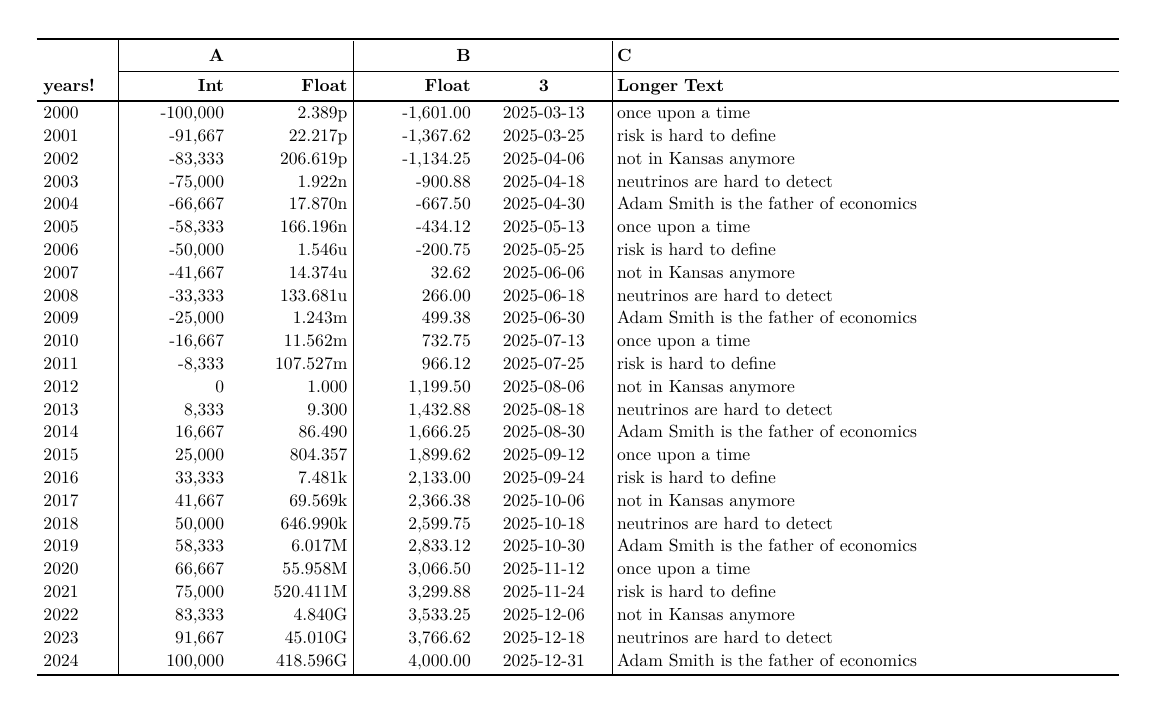
\begin{tikzpicture}[
    auto,
    transform shape,
    nosep/.style={inner sep=0},
    table/.style={
        matrix of nodes,
        row sep=0.125em,
        column sep=0.375em,
        nodes in empty cells,
        nodes={rectangle, scale=0.635, text badly ragged},
    row 1/.style={nodes={text=black, anchor=north, inner ysep=0, text height=0, text depth=0}},
    row 2/.style={nodes={text=black, anchor=south, inner ysep=.2em, minimum height=1.3em, font=\bfseries}},
    row 3/.style={nodes={text=black, anchor=south, inner ysep=.2em, minimum height=1.3em, font=\bfseries}},
    column  1/.style={nodes={align=left  }, text height=0.9em, text depth=0.2em, inner xsep=0.375em, inner ysep=0, text width=3.60em},
    column  2/.style={nodes={align=right }, nosep, text width=5.71em},
    column  3/.style={nodes={align=right }, nosep, text width=6.43em},
    column  4/.style={nodes={align=right }, nosep, text width=6.43em},
    column  5/.style={nodes={align=center}, nosep, text width=7.14em},
    column  6/.style={nodes={align=left  }, nosep, text width=27.85em},
    column  7/.style={text height=0.9em, text depth=0.2em, nosep, text width=0em}   }]
\matrix (TAZP6SDZPBHM6) [table, ampersand replacement=\&]{
      \&          \&           \&           \&            \&                                         \& \\
 \grtspacer \& A\grtspacer \& \grtspacer \& B\grtspacer \& \grtspacer \& C\grtspacer                             \& \\
 years!\grtspacer \& Int\grtspacer \& Float\grtspacer \& Float\grtspacer \& 3\grtspacer \& Longer Text\grtspacer                   \& \\
 2000 \& -100,000 \&    2.389p \& -1,601.00 \& 2025-03-13 \& once upon a time                        \& \\
 2001 \&  -91,667 \&   22.217p \& -1,367.62 \& 2025-03-25 \&  risk is hard to define                 \& \\
 2002 \&  -83,333 \&  206.619p \& -1,134.25 \& 2025-04-06 \&  not in Kansas anymore                  \& \\
 2003 \&  -75,000 \&    1.922n \&   -900.88 \& 2025-04-18 \&  neutrinos are hard to detect           \& \\
 2004 \&  -66,667 \&   17.870n \&   -667.50 \& 2025-04-30 \&   Adam Smith is the father of economics \& \\
 2005 \&  -58,333 \&  166.196n \&   -434.12 \& 2025-05-13 \& once upon a time                        \& \\
 2006 \&  -50,000 \&    1.546u \&   -200.75 \& 2025-05-25 \&  risk is hard to define                 \& \\
 2007 \&  -41,667 \&   14.374u \&     32.62 \& 2025-06-06 \&  not in Kansas anymore                  \& \\
 2008 \&  -33,333 \&  133.681u \&    266.00 \& 2025-06-18 \&  neutrinos are hard to detect           \& \\
 2009 \&  -25,000 \&    1.243m \&    499.38 \& 2025-06-30 \&   Adam Smith is the father of economics \& \\
 2010 \&  -16,667 \&   11.562m \&    732.75 \& 2025-07-13 \& once upon a time                        \& \\
 2011 \&   -8,333 \&  107.527m \&    966.12 \& 2025-07-25 \&  risk is hard to define                 \& \\
 2012 \&        0 \&     1.000 \&  1,199.50 \& 2025-08-06 \&  not in Kansas anymore                  \& \\
 2013 \&    8,333 \&     9.300 \&  1,432.88 \& 2025-08-18 \&  neutrinos are hard to detect           \& \\
 2014 \&   16,667 \&    86.490 \&  1,666.25 \& 2025-08-30 \&   Adam Smith is the father of economics \& \\
 2015 \&   25,000 \&   804.357 \&  1,899.62 \& 2025-09-12 \& once upon a time                        \& \\
 2016 \&   33,333 \&    7.481k \&  2,133.00 \& 2025-09-24 \&  risk is hard to define                 \& \\
 2017 \&   41,667 \&   69.569k \&  2,366.38 \& 2025-10-06 \&  not in Kansas anymore                  \& \\
 2018 \&   50,000 \&  646.990k \&  2,599.75 \& 2025-10-18 \&  neutrinos are hard to detect           \& \\
 2019 \&   58,333 \&    6.017M \&  2,833.12 \& 2025-10-30 \&   Adam Smith is the father of economics \& \\
 2020 \&   66,667 \&   55.958M \&  3,066.50 \& 2025-11-12 \& once upon a time                        \& \\
 2021 \&   75,000 \&  520.411M \&  3,299.88 \& 2025-11-24 \&  risk is hard to define                 \& \\
 2022 \&   83,333 \&    4.840G \&  3,533.25 \& 2025-12-06 \&  not in Kansas anymore                  \& \\
 2023 \&   91,667 \&   45.010G \&  3,766.62 \& 2025-12-18 \&  neutrinos are hard to detect           \& \\
 2024 \&  100,000 \&  418.596G \&  4,000.00 \& 2025-12-31 \&   Adam Smith is the father of economics \& \\
};

\path[draw, thick] (TAZP6SDZPBHM6-1-1.south west)  -- (TAZP6SDZPBHM6-1-7.south east);
\path[draw, semithick] ([yshift=-0.0625em]TAZP6SDZPBHM6-3-1.south west)  -- ([yshift=-0.0625em]TAZP6SDZPBHM6-3-7.south east);
\path[draw, thick] ([yshift=-0.3125em]TAZP6SDZPBHM6-28-1.base west)  -- ([yshift=-0.3125em]TAZP6SDZPBHM6-28-7.base east);
\path[draw, very thin] ([xshift=-0.1875em, yshift=-0.0625em]TAZP6SDZPBHM6-2-2.south west)  -- ([yshift=-0.0625em]TAZP6SDZPBHM6-2-7.south east);
\path[draw, very thin] ([xshift=-0.1875em]TAZP6SDZPBHM6-1-2.south west)  -- ([yshift=-0.3125em, xshift=-0.1875em]TAZP6SDZPBHM6-28-2.base west);
\path[draw, ultra thin] ([xshift=0.1875em, yshift=-0.0625em]TAZP6SDZPBHM6-1-3.south east)  -- ([yshift=-0.3125em, xshift=0.1875em]TAZP6SDZPBHM6-28-3.base east);
\path[draw, ultra thin] ([xshift=0.1875em, yshift=-0.0625em]TAZP6SDZPBHM6-1-5.south east)  -- ([yshift=-0.3125em, xshift=0.1875em]TAZP6SDZPBHM6-28-5.base east);



\end{tikzpicture}

\end{table}%

Illustrate some alternatives.

\begin{Shaded}
\begin{Highlighting}[]
\InformationTok{\textasciigrave{}\textasciigrave{}\textasciigrave{}\{python\}}
\InformationTok{\#| label: tbl{-}hard{-}rules{-}3}
\InformationTok{\#| tbl{-}cap: Quarto generated caption}

\InformationTok{display(sGT(hard.sample(5).sort\_index(), \textquotesingle{}No v rules, but h rules\textquotesingle{},}
\InformationTok{        vrule\_widths=(0,0,0),}
\InformationTok{        hrule\_widths=(1,0,0)))}

\InformationTok{display(sGT(hard.sample(5).sort\_index(),}
\InformationTok{        \textquotesingle{}Change default date and integer formats\textquotesingle{},}
\InformationTok{        default\_date\_str=\textquotesingle{}\%m{-}\%d\textquotesingle{}, default\_integer\_str=\textquotesingle{}[\{x:d\}]\textquotesingle{}))}

\InformationTok{display(sGT(hard.sample(5).sort\_index(),}
\InformationTok{        \textquotesingle{}Change padding, debug mode lines\textquotesingle{},}
\InformationTok{        default\_date\_str=\textquotesingle{}\%m{-}\%d\textquotesingle{}, default\_integer\_str=\textquotesingle{}[\{x:d\}]\textquotesingle{},}
\InformationTok{        padding\_trbl=(10, 10, 20, 20), debug=True))}
\InformationTok{\textasciigrave{}\textasciigrave{}\textasciigrave{}}
\end{Highlighting}
\end{Shaded}

\begin{table}

\caption{\label{tbl-hard-rules-3}Quarto generated caption}

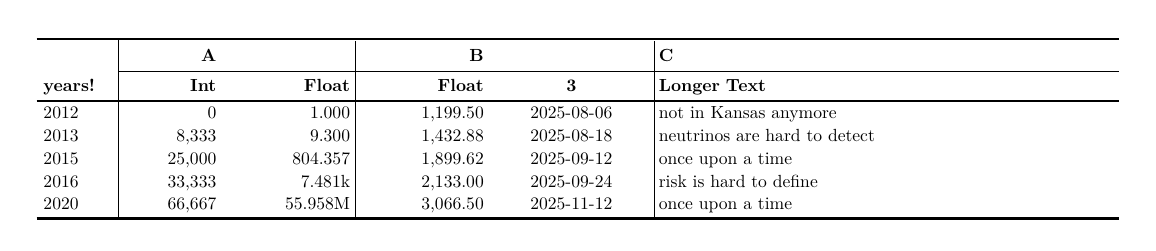
\begin{tikzpicture}[
    auto,
    transform shape,
    nosep/.style={inner sep=0},
    table/.style={
        matrix of nodes,
        row sep=0.125em,
        column sep=0.375em,
        nodes in empty cells,
        nodes={rectangle, scale=0.635, text badly ragged},
    row 1/.style={nodes={text=black, anchor=north, inner ysep=0, text height=0, text depth=0}},
    row 2/.style={nodes={text=black, anchor=south, inner ysep=.2em, minimum height=1.3em, font=\bfseries}},
    row 3/.style={nodes={text=black, anchor=south, inner ysep=.2em, minimum height=1.3em, font=\bfseries}},
    column  1/.style={nodes={align=left  }, text height=0.9em, text depth=0.2em, inner xsep=0.375em, inner ysep=0, text width=3.60em},
    column  2/.style={nodes={align=right }, nosep, text width=5.27em},
    column  3/.style={nodes={align=right }, nosep, text width=7.02em},
    column  4/.style={nodes={align=right }, nosep, text width=7.02em},
    column  5/.style={nodes={align=center}, nosep, text width=8.78em},
    column  6/.style={nodes={align=left  }, nosep, text width=25.46em},
    column  7/.style={text height=0.9em, text depth=0.2em, nosep, text width=0em}   }]
\matrix (TXF2KET77UF7H) [table, ampersand replacement=\&]{
      \&        \&          \&          \&            \&                               \& \\
 \grtspacer \& A\grtspacer \& \grtspacer \& B\grtspacer \& \grtspacer \& C\grtspacer                   \& \\
 years!\grtspacer \& Int\grtspacer \& Float\grtspacer \& Float\grtspacer \& 3\grtspacer \& Longer Text\grtspacer         \& \\
 2012 \&      0 \&    1.000 \& 1,199.50 \& 2025-08-06 \&  not in Kansas anymore        \& \\
 2013 \&  8,333 \&    9.300 \& 1,432.88 \& 2025-08-18 \&  neutrinos are hard to detect \& \\
 2015 \& 25,000 \&  804.357 \& 1,899.62 \& 2025-09-12 \& once upon a time              \& \\
 2016 \& 33,333 \&   7.481k \& 2,133.00 \& 2025-09-24 \&  risk is hard to define       \& \\
 2020 \& 66,667 \&  55.958M \& 3,066.50 \& 2025-11-12 \& once upon a time              \& \\
};

\path[draw, thick] (TXF2KET77UF7H-1-1.south west)  -- (TXF2KET77UF7H-1-7.south east);
\path[draw, semithick] ([yshift=-0.0625em]TXF2KET77UF7H-3-1.south west)  -- ([yshift=-0.0625em]TXF2KET77UF7H-3-7.south east);
\path[draw, thick] ([yshift=-0.3125em]TXF2KET77UF7H-8-1.base west)  -- ([yshift=-0.3125em]TXF2KET77UF7H-8-7.base east);
\path[draw, very thin] ([xshift=-0.1875em, yshift=-0.0625em]TXF2KET77UF7H-2-2.south west)  -- ([yshift=-0.0625em]TXF2KET77UF7H-2-7.south east);
\path[draw, very thin] ([xshift=-0.1875em]TXF2KET77UF7H-1-2.south west)  -- ([yshift=-0.3125em, xshift=-0.1875em]TXF2KET77UF7H-8-2.base west);
\path[draw, ultra thin] ([xshift=0.1875em, yshift=-0.0625em]TXF2KET77UF7H-1-3.south east)  -- ([yshift=-0.3125em, xshift=0.1875em]TXF2KET77UF7H-8-3.base east);
\path[draw, ultra thin] ([xshift=0.1875em, yshift=-0.0625em]TXF2KET77UF7H-1-5.south east)  -- ([yshift=-0.3125em, xshift=0.1875em]TXF2KET77UF7H-8-5.base east);



\end{tikzpicture}

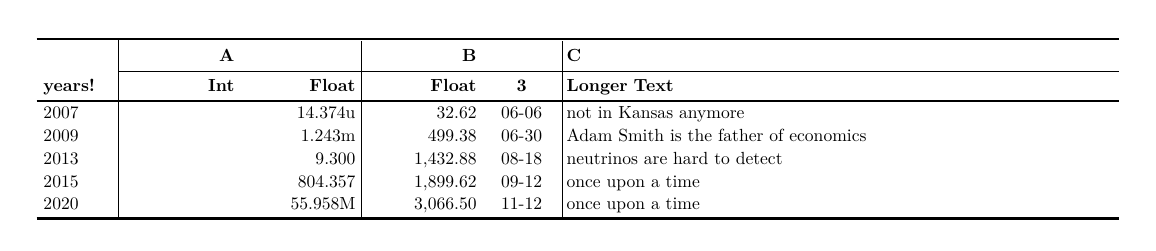
\begin{tikzpicture}[
    auto,
    transform shape,
    nosep/.style={inner sep=0},
    table/.style={
        matrix of nodes,
        row sep=0.125em,
        column sep=0.375em,
        nodes in empty cells,
        nodes={rectangle, scale=0.635, text badly ragged},
    row 1/.style={nodes={text=black, anchor=north, inner ysep=0, text height=0, text depth=0}},
    row 2/.style={nodes={text=black, anchor=south, inner ysep=.2em, minimum height=1.3em, font=\bfseries}},
    row 3/.style={nodes={text=black, anchor=south, inner ysep=.2em, minimum height=1.3em, font=\bfseries}},
    column  1/.style={nodes={align=left  }, text height=0.9em, text depth=0.2em, inner xsep=0.375em, inner ysep=0, text width=3.60em},
    column  2/.style={nodes={align=right }, nosep, text width=6.30em},
    column  3/.style={nodes={align=right }, nosep, text width=6.30em},
    column  4/.style={nodes={align=right }, nosep, text width=6.30em},
    column  5/.style={nodes={align=center}, nosep, text width=3.94em},
    column  6/.style={nodes={align=left  }, nosep, text width=30.71em},
    column  7/.style={text height=0.9em, text depth=0.2em, nosep, text width=0em}   }]
\matrix (TTHJZXEFZS7PW) [table, ampersand replacement=\&]{
      \&          \&          \&          \&       \&                                         \& \\
 \grtspacer \& A\grtspacer \& \grtspacer \& B\grtspacer \& \grtspacer \& C\grtspacer                             \& \\
 years!\grtspacer \& Int\grtspacer \& Float\grtspacer \& Float\grtspacer \& 3\grtspacer \& Longer Text\grtspacer                   \& \\
 2007 \& [-41667] \&  14.374u \&    32.62 \& 06-06 \&  not in Kansas anymore                  \& \\
 2009 \& [-25000] \&   1.243m \&   499.38 \& 06-30 \&   Adam Smith is the father of economics \& \\
 2013 \&   [8333] \&    9.300 \& 1,432.88 \& 08-18 \&  neutrinos are hard to detect           \& \\
 2015 \&  [25000] \&  804.357 \& 1,899.62 \& 09-12 \& once upon a time                        \& \\
 2020 \&  [66667] \&  55.958M \& 3,066.50 \& 11-12 \& once upon a time                        \& \\
};

\path[draw, thick] (TTHJZXEFZS7PW-1-1.south west)  -- (TTHJZXEFZS7PW-1-7.south east);
\path[draw, semithick] ([yshift=-0.0625em]TTHJZXEFZS7PW-3-1.south west)  -- ([yshift=-0.0625em]TTHJZXEFZS7PW-3-7.south east);
\path[draw, thick] ([yshift=-0.3125em]TTHJZXEFZS7PW-8-1.base west)  -- ([yshift=-0.3125em]TTHJZXEFZS7PW-8-7.base east);
\path[draw, very thin] ([xshift=-0.1875em, yshift=-0.0625em]TTHJZXEFZS7PW-2-2.south west)  -- ([yshift=-0.0625em]TTHJZXEFZS7PW-2-7.south east);
\path[draw, very thin] ([xshift=-0.1875em]TTHJZXEFZS7PW-1-2.south west)  -- ([yshift=-0.3125em, xshift=-0.1875em]TTHJZXEFZS7PW-8-2.base west);
\path[draw, ultra thin] ([xshift=0.1875em, yshift=-0.0625em]TTHJZXEFZS7PW-1-3.south east)  -- ([yshift=-0.3125em, xshift=0.1875em]TTHJZXEFZS7PW-8-3.base east);
\path[draw, ultra thin] ([xshift=0.1875em, yshift=-0.0625em]TTHJZXEFZS7PW-1-5.south east)  -- ([yshift=-0.3125em, xshift=0.1875em]TTHJZXEFZS7PW-8-5.base east);



\end{tikzpicture}

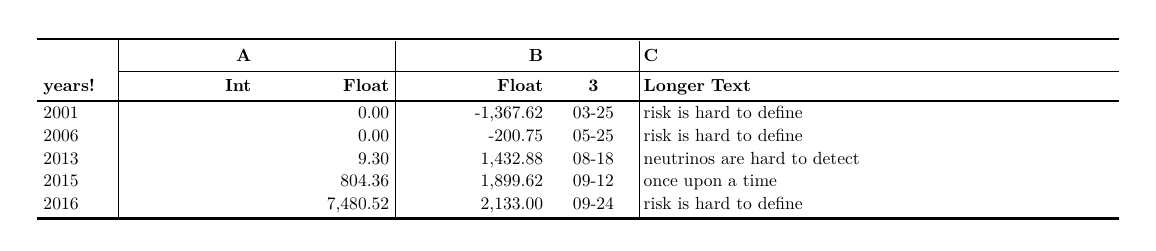
\begin{tikzpicture}[
    auto,
    transform shape,
    nosep/.style={inner sep=0},
    table/.style={
        matrix of nodes,
        row sep=0.125em,
        column sep=0.375em,
        nodes in empty cells,
        nodes={rectangle, scale=0.635, text badly ragged},
    row 1/.style={nodes={text=black, anchor=north, inner ysep=0, text height=0, text depth=0}},
    row 2/.style={nodes={text=black, anchor=south, inner ysep=.2em, minimum height=1.3em, font=\bfseries}},
    row 3/.style={nodes={text=black, anchor=south, inner ysep=.2em, minimum height=1.3em, font=\bfseries}},
    column  1/.style={nodes={align=left  }, text height=0.9em, text depth=0.2em, inner xsep=0.375em, inner ysep=0, text width=3.60em},
    column  2/.style={nodes={align=right }, nosep, text width=7.26em},
    column  3/.style={nodes={align=right }, nosep, text width=7.26em},
    column  4/.style={nodes={align=right }, nosep, text width=8.17em},
    column  5/.style={nodes={align=center}, nosep, text width=4.54em},
    column  6/.style={nodes={align=left  }, nosep, text width=26.32em},
    column  7/.style={text height=0.9em, text depth=0.2em, nosep, text width=0em}   }]
\matrix (T4YPCZZ75IBAL) [table, ampersand replacement=\&]{
      \&          \&          \&           \&       \&                               \& \\
 \grtspacer \& A\grtspacer \& \grtspacer \& B\grtspacer \& \grtspacer \& C\grtspacer                   \& \\
 years!\grtspacer \& Int\grtspacer \& Float\grtspacer \& Float\grtspacer \& 3\grtspacer \& Longer Text\grtspacer         \& \\
 2001 \& [-91667] \&     0.00 \& -1,367.62 \& 03-25 \&  risk is hard to define       \& \\
 2006 \& [-50000] \&     0.00 \&   -200.75 \& 05-25 \&  risk is hard to define       \& \\
 2013 \&   [8333] \&     9.30 \&  1,432.88 \& 08-18 \&  neutrinos are hard to detect \& \\
 2015 \&  [25000] \&   804.36 \&  1,899.62 \& 09-12 \& once upon a time              \& \\
 2016 \&  [33333] \& 7,480.52 \&  2,133.00 \& 09-24 \&  risk is hard to define       \& \\
};

\path[draw, thick] (T4YPCZZ75IBAL-1-1.south west)  -- (T4YPCZZ75IBAL-1-7.south east);
\path[draw, semithick] ([yshift=-0.0625em]T4YPCZZ75IBAL-3-1.south west)  -- ([yshift=-0.0625em]T4YPCZZ75IBAL-3-7.south east);
\path[draw, thick] ([yshift=-0.3125em]T4YPCZZ75IBAL-8-1.base west)  -- ([yshift=-0.3125em]T4YPCZZ75IBAL-8-7.base east);
\path[draw, very thin] ([xshift=-0.1875em, yshift=-0.0625em]T4YPCZZ75IBAL-2-2.south west)  -- ([yshift=-0.0625em]T4YPCZZ75IBAL-2-7.south east);
\path[draw, very thin] ([xshift=-0.1875em]T4YPCZZ75IBAL-1-2.south west)  -- ([yshift=-0.3125em, xshift=-0.1875em]T4YPCZZ75IBAL-8-2.base west);
\path[draw, ultra thin] ([xshift=0.1875em, yshift=-0.0625em]T4YPCZZ75IBAL-1-3.south east)  -- ([yshift=-0.3125em, xshift=0.1875em]T4YPCZZ75IBAL-8-3.base east);
\path[draw, ultra thin] ([xshift=0.1875em, yshift=-0.0625em]T4YPCZZ75IBAL-1-5.south east)  -- ([yshift=-0.3125em, xshift=0.1875em]T4YPCZZ75IBAL-8-5.base east);



\end{tikzpicture}

\end{table}%

Here is the raw output.

\footnotesize

\phantomsection\label{raw-output}
\begin{Shaded}
\begin{Highlighting}[]
\NormalTok{f }\OperatorTok{=}\NormalTok{ sGT(hard.head(}\DecValTok{4}\NormalTok{), debug}\OperatorTok{=}\VariableTok{True}\NormalTok{)}
\BuiltInTok{print}\NormalTok{(}\StringTok{\textquotesingle{}HTML output}\CharTok{\textbackslash{}n}\StringTok{\textquotesingle{}}\NormalTok{)}
\BuiltInTok{print}\NormalTok{(f.\_repr\_html\_())}

\BuiltInTok{print}\NormalTok{(}\StringTok{\textquotesingle{}}\CharTok{\textbackslash{}n\textbackslash{}n\textbackslash{}n}\StringTok{TeX output}\CharTok{\textbackslash{}n}\StringTok{\textquotesingle{}}\NormalTok{)}
\BuiltInTok{print}\NormalTok{(f.\_repr\_latex\_())}
\end{Highlighting}
\end{Shaded}

\begin{verbatim}
HTML output

<div class="greater-table">
<style>
    #T4HD5XXJXVBZO  {
    border-collapse: collapse;
    font-family: "Roboto", "Open Sans Condensed", "Arial", 'Segoe UI', sans-serif;
    font-size: 0.9em;
    width: auto;
    border: none;
    overflow: auto;
    }
    /* tag formats */
    #T4HD5XXJXVBZO caption {
        padding: 8px 10px 4px 10px;
        font-size: 0.99em;
        text-align: center;
        font-weight: normal;
        caption-side: top;
    }
    #T4HD5XXJXVBZO thead {
        /* top and bottom of header */
        border-top: 1px solid #0ff;
        border-bottom: 1px solid #0ff;
        font-size: 0.99em;
        }
    #T4HD5XXJXVBZO tbody {
        /* bottom of body */
        border-bottom: 1px solid #f0f;
        }
    #T4HD5XXJXVBZO th  {
        vertical-align: bottom;
        padding: 8px 10px 8px 10px;
    }
    #T4HD5XXJXVBZO td {
        /* top, right, bottom left cell padding */
        padding: 4px 10px 4px 10px;
        vertical-align: top;
    }
    /* class overrides */
    #T4HD5XXJXVBZO .grt-hrule-0 {
        border-top: 0px solid #f00;
    }
    #T4HD5XXJXVBZO .grt-hrule-1 {
        border-top: 0px solid #b00;
    }
    #T4HD5XXJXVBZO .grt-hrule-2 {
        border-top: 0px solid #900;
    }
    /* for the header, there if you have v lines you want h lines
       hence use vrule_widths */
    #T4HD5XXJXVBZO .grt-bhrule-0 {
        border-bottom: 1.5px solid #f00;
    }
    #T4HD5XXJXVBZO .grt-bhrule-1 {
        border-bottom: 1px solid #b00;
    }
    #T4HD5XXJXVBZO .grt-vrule-index {
        border-left: 1.5px solid #0f0;
    }
    #T4HD5XXJXVBZO .grt-vrule-0 {
        border-left: 1.5px solid #0f0;
    }
    #T4HD5XXJXVBZO .grt-vrule-1 {
        border-left: 1px solid #0a0;
    }
    #T4HD5XXJXVBZO .grt-vrule-2 {
        border-left: 0.5px solid #090;
    }
    #T4HD5XXJXVBZO .grt-left {
        text-align: left;
    }
    #T4HD5XXJXVBZO .grt-center {
        text-align: center;
    }
    #T4HD5XXJXVBZO .grt-right {
        text-align: right;
        font-variant-numeric: tabular-nums;
    }
    #T4HD5XXJXVBZO .grt-head {
        font-family: "Times New Roman", 'Courier New';
        font-size: 0.99em;
    }
    #T4HD5XXJXVBZO .grt-bold {
        font-weight: bold;
    }
</style>
<table id="T4HD5XXJXVBZO">
<caption> (id: T4HD5XXJXVBZO)</caption>
<thead>
<tr>
<th class="grt-left"></th>
<th class="grt-center grt-bhrule-0 grt-vrule-index" colspan="2">A</th>
<th class="grt-center grt-bhrule-0 grt-vrule-0" colspan="2">B</th>
<th class="grt-center grt-bhrule-0 grt-vrule-0" colspan="1">C</th>
</tr>
<tr>
<th class="grt-left">years!</th>
<th class="grt-center grt-vrule-index" colspan="1">Int</th>
<th class="grt-center grt-vrule-1" colspan="1">Float</th>
<th class="grt-center grt-vrule-0" colspan="1">Float</th>
<th class="grt-center grt-vrule-1" colspan="1">3</th>
<th class="grt-center grt-vrule-0" colspan="1">Longer Text</th>
</tr>
</thead>
<tbody>
<tr>
<td class="grt-left">2000</td>
<td class="grt-right grt-vrule-index">-100,000</td>
<td class="grt-right grt-vrule-1"> 2.389p</td>
<td class="grt-right grt-vrule-0">-1,601.00</td>
<td class="grt-center grt-vrule-1">2025-03-13</td>
<td class="grt-left grt-vrule-0">once upon a time</td>
</tr>
<tr>
<td class="grt-left grt-hrule-0">2001</td>
<td class="grt-right grt-hrule-0 grt-vrule-index">-91,667</td>
<td class="grt-right grt-hrule-0 grt-vrule-1"> 22.217p</td>
<td class="grt-right grt-hrule-0 grt-vrule-0">-1,367.62</td>
<td class="grt-center grt-hrule-0 grt-vrule-1">2025-03-25</td>
<td class="grt-left grt-hrule-0 grt-vrule-0"> risk is hard to define</td>
</tr>
<tr>
<td class="grt-left grt-hrule-0">2002</td>
<td class="grt-right grt-hrule-0 grt-vrule-index">-83,333</td>
<td class="grt-right grt-hrule-0 grt-vrule-1"> 206.619p</td>
<td class="grt-right grt-hrule-0 grt-vrule-0">-1,134.25</td>
<td class="grt-center grt-hrule-0 grt-vrule-1">2025-04-06</td>
<td class="grt-left grt-hrule-0 grt-vrule-0"> not in Kansas anymore</td>
</tr>
<tr>
<td class="grt-left grt-hrule-0">2003</td>
<td class="grt-right grt-hrule-0 grt-vrule-index">-75,000</td>
<td class="grt-right grt-hrule-0 grt-vrule-1"> 1.922n</td>
<td class="grt-right grt-hrule-0 grt-vrule-0">-900.88</td>
<td class="grt-center grt-hrule-0 grt-vrule-1">2025-04-18</td>
<td class="grt-left grt-hrule-0 grt-vrule-0"> neutrinos are hard to detect</td>
</tr>
</tbody>
</table></div>



TeX output


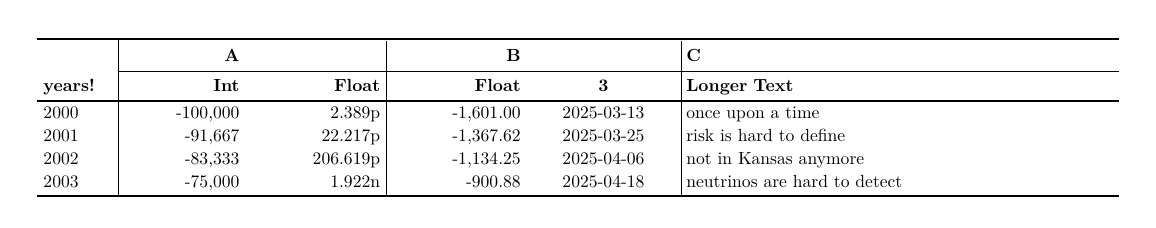
\begin{tikzpicture}[
    auto,
    transform shape,
    nosep/.style={inner sep=0},
    table/.style={
        matrix of nodes,
        row sep=0.125em,
        column sep=0.375em,
        nodes in empty cells,
        nodes={rectangle, scale=0.635, text badly ragged},
    row 1/.style={nodes={text=black, anchor=north, inner ysep=0, text height=0, text depth=0}},
    row 2/.style={nodes={text=black, anchor=south, inner ysep=.2em, minimum height=1.3em, font=\bfseries}},
    row 3/.style={nodes={text=black, anchor=south, inner ysep=.2em, minimum height=1.3em, font=\bfseries}},
    column  1/.style={nodes={align=left  }, text height=0.9em, text depth=0.2em, inner xsep=0.375em, inner ysep=0, text width=3.60em},
    column  2/.style={nodes={align=right }, nosep, text width=6.59em},
    column  3/.style={nodes={align=right }, nosep, text width=7.41em},
    column  4/.style={nodes={align=right }, nosep, text width=7.41em},
    column  5/.style={nodes={align=center}, nosep, text width=8.24em},
    column  6/.style={nodes={align=left  }, nosep, text width=23.89em},
    column  7/.style={text height=0.9em, text depth=0.2em, nosep, text width=0em}   }]
\matrix (T4HD5XXJXVBZO) [table, ampersand replacement=\&]{
      \&          \&           \&           \&            \&                               \& \\
 \grtspacer \& A\grtspacer \& \grtspacer \& B\grtspacer \& \grtspacer \& C\grtspacer                   \& \\
 years!\grtspacer \& Int\grtspacer \& Float\grtspacer \& Float\grtspacer \& 3\grtspacer \& Longer Text\grtspacer         \& \\
 2000 \& -100,000 \&    2.389p \& -1,601.00 \& 2025-03-13 \& once upon a time              \& \\
 2001 \&  -91,667 \&   22.217p \& -1,367.62 \& 2025-03-25 \&  risk is hard to define       \& \\
 2002 \&  -83,333 \&  206.619p \& -1,134.25 \& 2025-04-06 \&  not in Kansas anymore        \& \\
 2003 \&  -75,000 \&    1.922n \&   -900.88 \& 2025-04-18 \&  neutrinos are hard to detect \& \\
};

\path[draw, thick] (T4HD5XXJXVBZO-1-1.south west)  -- (T4HD5XXJXVBZO-1-7.south east);
\path[draw, semithick] ([yshift=-0.0625em]T4HD5XXJXVBZO-3-1.south west)  -- ([yshift=-0.0625em]T4HD5XXJXVBZO-3-7.south east);
\path[draw, thick] ([yshift=-0.3125em]T4HD5XXJXVBZO-7-1.base west)  -- ([yshift=-0.3125em]T4HD5XXJXVBZO-7-7.base east);
\path[draw, very thin] ([xshift=-0.1875em, yshift=-0.0625em]T4HD5XXJXVBZO-2-2.south west)  -- ([yshift=-0.0625em]T4HD5XXJXVBZO-2-7.south east);
\path[draw, very thin] ([xshift=-0.1875em]T4HD5XXJXVBZO-1-2.south west)  -- ([yshift=-0.3125em, xshift=-0.1875em]T4HD5XXJXVBZO-7-2.base west);
\path[draw, ultra thin] ([xshift=0.1875em, yshift=-0.0625em]T4HD5XXJXVBZO-1-3.south east)  -- ([yshift=-0.3125em, xshift=0.1875em]T4HD5XXJXVBZO-7-3.base east);
\path[draw, ultra thin] ([xshift=0.1875em, yshift=-0.0625em]T4HD5XXJXVBZO-1-5.south east)  -- ([yshift=-0.3125em, xshift=0.1875em]T4HD5XXJXVBZO-7-5.base east);



\end{tikzpicture}
\end{verbatim}

\normalsize

\section{A Table with TeX}\label{a-table-with-tex}

\begin{Shaded}
\begin{Highlighting}[]
\NormalTok{index }\OperatorTok{=}\NormalTok{ pd.Index([}\StringTok{"A"}\NormalTok{, }\StringTok{"B"}\NormalTok{, }\StringTok{"$C\_1$"}\NormalTok{, }\StringTok{"C\_2 not tex"}\NormalTok{, }\StringTok{\textquotesingle{}$}\CharTok{\textbackslash{}\textbackslash{}}\StringTok{cos(A)$\textquotesingle{}}\NormalTok{])}
\NormalTok{tex }\OperatorTok{=}\NormalTok{ pd.DataFrame(}
\NormalTok{\{}\StringTok{\textquotesingle{}x\textquotesingle{}}\NormalTok{: np.arange(}\DecValTok{2020}\NormalTok{, }\DecValTok{2025}\NormalTok{, dtype}\OperatorTok{=}\BuiltInTok{int}\NormalTok{),}
\StringTok{\textquotesingle{}b\textquotesingle{}}\NormalTok{: np.random.random(}\DecValTok{5}\NormalTok{),}
\StringTok{\textquotesingle{}a1\textquotesingle{}}\NormalTok{: [}\SpecialStringTok{f\textquotesingle{}$x\^{}}\SpecialCharTok{\{}\NormalTok{i}\SpecialCharTok{\}}\SpecialStringTok{$\textquotesingle{}} \ControlFlowTok{for}\NormalTok{ i }\KeywordTok{in} \BuiltInTok{range}\NormalTok{(}\DecValTok{5}\NormalTok{,}\DecValTok{10}\NormalTok{)],}
\StringTok{\textquotesingle{}a2\textquotesingle{}}\NormalTok{: [}\SpecialStringTok{f\textquotesingle{}$}\CharTok{\textbackslash{}\textbackslash{}}\SpecialStringTok{sin(}\SpecialCharTok{\{}\NormalTok{i}\SpecialCharTok{\}}\SpecialStringTok{x}\CharTok{\textbackslash{}\textbackslash{}}\SpecialStringTok{pi/n)$\textquotesingle{}} \ControlFlowTok{for}\NormalTok{ i }\KeywordTok{in} \BuiltInTok{range}\NormalTok{(}\DecValTok{5}\NormalTok{,}\DecValTok{10}\NormalTok{)],}
\StringTok{\textquotesingle{}a3\textquotesingle{}}\NormalTok{: [}\SpecialStringTok{f\textquotesingle{}$x\^{}}\SpecialCharTok{\{}\NormalTok{i}\SpecialCharTok{\}}\SpecialStringTok{$\textquotesingle{}} \ControlFlowTok{for}\NormalTok{ i }\KeywordTok{in} \BuiltInTok{range}\NormalTok{(}\DecValTok{5}\NormalTok{,}\DecValTok{10}\NormalTok{)],}
\StringTok{\textquotesingle{}a4\textquotesingle{}}\NormalTok{: [}\SpecialStringTok{f\textquotesingle{}}\CharTok{\textbackslash{}\textbackslash{}}\SpecialStringTok{(x\^{}}\SpecialCharTok{\{}\NormalTok{i}\SpecialCharTok{\}}\CharTok{\textbackslash{}\textbackslash{}}\SpecialStringTok{)\textquotesingle{}} \ControlFlowTok{for}\NormalTok{ i }\KeywordTok{in} \BuiltInTok{range}\NormalTok{(}\DecValTok{5}\NormalTok{,}\DecValTok{10}\NormalTok{)],}
\NormalTok{\}).set\_index(}\StringTok{\textquotesingle{}x\textquotesingle{}}\NormalTok{)}
\NormalTok{tex }\OperatorTok{=}\NormalTok{ tex.head()}
\NormalTok{tex.columns }\OperatorTok{=}\NormalTok{ index}
\NormalTok{tex}
\end{Highlighting}
\end{Shaded}

\begin{longtable}[]{@{}llllll@{}}

\caption{\label{tbl-tex}Quarto generated caption: table displayed by
default routine.}

\tabularnewline

\toprule\noalign{}
& A & B & \$C\_1\$ & C\_2 not tex & \$\textbackslash cos(A)\$ \\
x & & & & & \\
\midrule\noalign{}
\endhead
\bottomrule\noalign{}
\endlastfoot
2020 & 0.324114 & \$x\^{}5\$ &
\$\textbackslash sin(5x\textbackslash pi/n)\$ & \$x\^{}5\$ &
\textbackslash(x\^{}5\textbackslash) \\
2021 & 0.213173 & \$x\^{}6\$ &
\$\textbackslash sin(6x\textbackslash pi/n)\$ & \$x\^{}6\$ &
\textbackslash(x\^{}6\textbackslash) \\
2022 & 0.639189 & \$x\^{}7\$ &
\$\textbackslash sin(7x\textbackslash pi/n)\$ & \$x\^{}7\$ &
\textbackslash(x\^{}7\textbackslash) \\
2023 & 0.112127 & \$x\^{}8\$ &
\$\textbackslash sin(8x\textbackslash pi/n)\$ & \$x\^{}8\$ &
\textbackslash(x\^{}8\textbackslash) \\
2024 & 0.681293 & \$x\^{}9\$ &
\$\textbackslash sin(9x\textbackslash pi/n)\$ & \$x\^{}9\$ &
\textbackslash(x\^{}9\textbackslash) \\

\end{longtable}

\begin{Shaded}
\begin{Highlighting}[]
\NormalTok{sGT(tex, }\StringTok{\textquotesingle{}GT Caption\textquotesingle{}}\NormalTok{)}
\end{Highlighting}
\end{Shaded}

\begin{table}

\caption{\label{tbl-tex-2}Quarto generated caption}

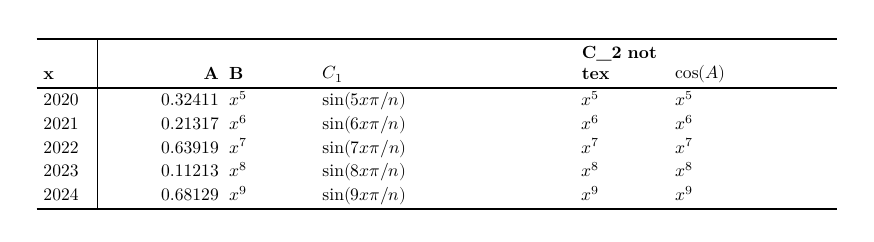
\begin{tikzpicture}[
    auto,
    transform shape,
    nosep/.style={inner sep=0},
    table/.style={
        matrix of nodes,
        row sep=0.125em,
        column sep=0.375em,
        nodes in empty cells,
        nodes={rectangle, scale=0.635, text badly ragged},
    row 1/.style={nodes={text=black, anchor=north, inner ysep=0, text height=0, text depth=0}},
    row 2/.style={nodes={text=black, anchor=south, inner ysep=.2em, minimum height=1.3em, font=\bfseries}},
    column  1/.style={nodes={align=left  }, text height=0.9em, text depth=0.2em, inner xsep=0.375em, inner ysep=0, text width=2.40em},
    column  2/.style={nodes={align=right }, nosep, text width=6.61em},
    column  3/.style={nodes={align=left  }, nosep, text width=4.72em},
    column  4/.style={nodes={align=left  }, nosep, text width=14.17em},
    column  5/.style={nodes={align=left  }, nosep, text width=4.72em},
    column  6/.style={nodes={align=left  }, nosep, text width=8.50em},
    column  7/.style={text height=0.9em, text depth=0.2em, nosep, text width=0em}   }]
\matrix (TYTHIEOF4LT3H) [table, ampersand replacement=\&]{
      \&         \&       \&                 \&       \&         \& \\
 x\grtspacer \& A\grtspacer \& B\grtspacer \& $C_1$\grtspacer \& C\_2 not tex\grtspacer \& $\cos(A)$\grtspacer \& \\
 2020 \& 0.32411 \& $x^5$ \& $\sin(5x\pi/n)$ \& $x^5$ \& \(x^5\) \& \\
 2021 \& 0.21317 \& $x^6$ \& $\sin(6x\pi/n)$ \& $x^6$ \& \(x^6\) \& \\
 2022 \& 0.63919 \& $x^7$ \& $\sin(7x\pi/n)$ \& $x^7$ \& \(x^7\) \& \\
 2023 \& 0.11213 \& $x^8$ \& $\sin(8x\pi/n)$ \& $x^8$ \& \(x^8\) \& \\
 2024 \& 0.68129 \& $x^9$ \& $\sin(9x\pi/n)$ \& $x^9$ \& \(x^9\) \& \\
};

\path[draw, thick] (TYTHIEOF4LT3H-1-1.south west)  -- (TYTHIEOF4LT3H-1-7.south east);
\path[draw, semithick] ([yshift=-0.0625em]TYTHIEOF4LT3H-2-1.south west)  -- ([yshift=-0.0625em]TYTHIEOF4LT3H-2-7.south east);
\path[draw, thick] ([yshift=-0.3125em]TYTHIEOF4LT3H-7-1.base west)  -- ([yshift=-0.3125em]TYTHIEOF4LT3H-7-7.base east);
\path[draw, very thin] ([xshift=-0.1875em]TYTHIEOF4LT3H-1-2.south west)  -- ([yshift=-0.3125em, xshift=-0.1875em]TYTHIEOF4LT3H-7-2.base west);



\end{tikzpicture}

\end{table}%

Ratio columns.

\begin{Shaded}
\begin{Highlighting}[]
\NormalTok{tex.columns }\OperatorTok{=}\NormalTok{ [}\StringTok{"A (\%)"}\NormalTok{, }\StringTok{"B"}\NormalTok{, }\StringTok{"$C\_1$"}\NormalTok{, }\StringTok{"C\_2 not tex"}\NormalTok{, }\StringTok{\textquotesingle{}$}\CharTok{\textbackslash{}\textbackslash{}}\StringTok{cos(A)$\textquotesingle{}}\NormalTok{]}
\NormalTok{sGT(tex, }\StringTok{\textquotesingle{}Ratio columns in A\textquotesingle{}}\NormalTok{, ratio\_cols}\OperatorTok{=}\StringTok{\textquotesingle{}A (\%)\textquotesingle{}}\NormalTok{)}
\end{Highlighting}
\end{Shaded}

\begin{table}

\caption{\label{tbl-tex-3}greater table output}

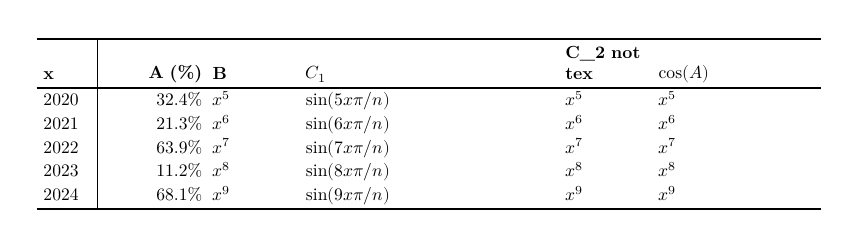
\begin{tikzpicture}[
    auto,
    transform shape,
    nosep/.style={inner sep=0},
    table/.style={
        matrix of nodes,
        row sep=0.125em,
        column sep=0.375em,
        nodes in empty cells,
        nodes={rectangle, scale=0.635, text badly ragged},
    row 1/.style={nodes={text=black, anchor=north, inner ysep=0, text height=0, text depth=0}},
    row 2/.style={nodes={text=black, anchor=south, inner ysep=.2em, minimum height=1.3em, font=\bfseries}},
    column  1/.style={nodes={align=left  }, text height=0.9em, text depth=0.2em, inner xsep=0.375em, inner ysep=0, text width=2.40em},
    column  2/.style={nodes={align=right }, nosep, text width=5.67em},
    column  3/.style={nodes={align=left  }, nosep, text width=4.72em},
    column  4/.style={nodes={align=left  }, nosep, text width=14.17em},
    column  5/.style={nodes={align=left  }, nosep, text width=4.72em},
    column  6/.style={nodes={align=left  }, nosep, text width=8.50em},
    column  7/.style={text height=0.9em, text depth=0.2em, nosep, text width=0em}   }]
\matrix (TUEYL75U3V6YO) [table, ampersand replacement=\&]{
      \&        \&       \&                 \&       \&         \& \\
 x\grtspacer \& A (\%)\grtspacer \& B\grtspacer \& $C_1$\grtspacer \& C\_2 not tex\grtspacer \& $\cos(A)$\grtspacer \& \\
 2020 \& 32.4\% \& $x^5$ \& $\sin(5x\pi/n)$ \& $x^5$ \& \(x^5\) \& \\
 2021 \& 21.3\% \& $x^6$ \& $\sin(6x\pi/n)$ \& $x^6$ \& \(x^6\) \& \\
 2022 \& 63.9\% \& $x^7$ \& $\sin(7x\pi/n)$ \& $x^7$ \& \(x^7\) \& \\
 2023 \& 11.2\% \& $x^8$ \& $\sin(8x\pi/n)$ \& $x^8$ \& \(x^8\) \& \\
 2024 \& 68.1\% \& $x^9$ \& $\sin(9x\pi/n)$ \& $x^9$ \& \(x^9\) \& \\
};

\path[draw, thick] (TUEYL75U3V6YO-1-1.south west)  -- (TUEYL75U3V6YO-1-7.south east);
\path[draw, semithick] ([yshift=-0.0625em]TUEYL75U3V6YO-2-1.south west)  -- ([yshift=-0.0625em]TUEYL75U3V6YO-2-7.south east);
\path[draw, thick] ([yshift=-0.3125em]TUEYL75U3V6YO-7-1.base west)  -- ([yshift=-0.3125em]TUEYL75U3V6YO-7-7.base east);
\path[draw, very thin] ([xshift=-0.1875em]TUEYL75U3V6YO-1-2.south west)  -- ([yshift=-0.3125em, xshift=-0.1875em]TUEYL75U3V6YO-7-2.base west);



\end{tikzpicture}

\end{table}%

\section{Greater\_tables Test Suite}\label{greater_tables-test-suite}

\phantomsection\label{greater-tables-test}
\begin{Shaded}
\begin{Highlighting}[]
\NormalTok{test\_gen }\OperatorTok{=}\NormalTok{ gtu.TestDFGenerator(}\DecValTok{0}\NormalTok{, }\DecValTok{0}\NormalTok{)}
\NormalTok{ans }\OperatorTok{=}\NormalTok{ test\_gen.test\_suite()    }
\end{Highlighting}
\end{Shaded}

\subsection{Test Table: basic}\label{test-table-basic}

\begin{Shaded}
\begin{Highlighting}[]
\NormalTok{hrw }\OperatorTok{=}\NormalTok{ (}\DecValTok{0}\NormalTok{, }\DecValTok{0}\NormalTok{, }\DecValTok{0}\NormalTok{)}
\NormalTok{sGT(ans[}\StringTok{\textquotesingle{}basic\textquotesingle{}}\NormalTok{], }\StringTok{"Basic"}\NormalTok{, ratio\_cols}\OperatorTok{=}\StringTok{\textquotesingle{}z\textquotesingle{}}\NormalTok{, aligners}\OperatorTok{=}\NormalTok{\{}\StringTok{\textquotesingle{}w\textquotesingle{}}\NormalTok{: }\StringTok{\textquotesingle{}l\textquotesingle{}}\NormalTok{\},}
\NormalTok{        hrule\_widths}\OperatorTok{=}\NormalTok{hrw)}
\end{Highlighting}
\end{Shaded}

\begin{table}

\caption{\label{tbl-greater-tables-test-0}Output for test table basic}

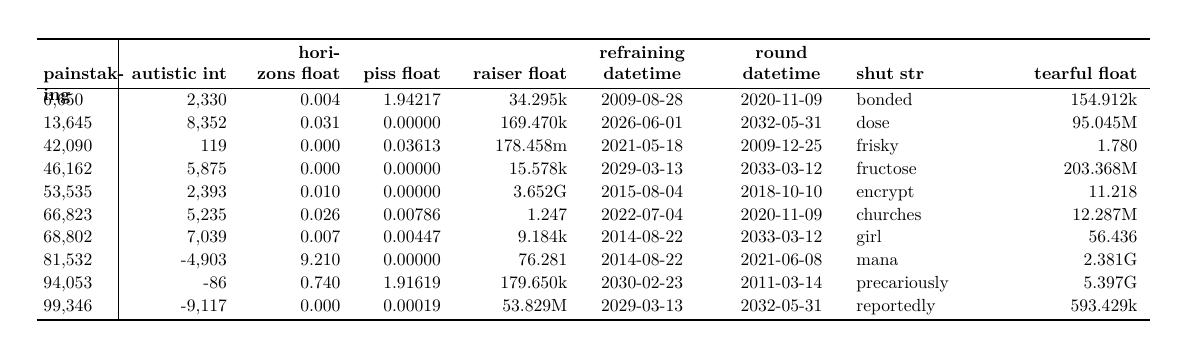
\begin{tikzpicture}[
    auto,
    transform shape,
    nosep/.style={inner sep=0},
    table/.style={
        matrix of nodes,
        row sep=0.125em,
        column sep=0.375em,
        nodes in empty cells,
        nodes={rectangle, scale=0.635, text badly ragged},
    row 1/.style={nodes={text=black, anchor=north, inner ysep=0, text height=0, text depth=0}},
    row 2/.style={nodes={text=black, anchor=south, inner ysep=.2em, minimum height=1.3em, font=\bfseries}},
    column  1/.style={nodes={align=left  }, text height=0.9em, text depth=0.2em, inner xsep=0.375em, inner ysep=0, text width=3.60em},
    column  2/.style={nodes={align=right }, nosep, text width=5.87em},
    column  3/.style={nodes={align=right }, nosep, text width=5.87em},
    column  4/.style={nodes={align=right }, nosep, text width=5.13em},
    column  5/.style={nodes={align=right }, nosep, text width=6.60em},
    column  6/.style={nodes={align=center}, nosep, text width=7.34em},
    column  7/.style={nodes={align=center}, nosep, text width=7.34em},
    column  8/.style={nodes={align=left  }, nosep, text width=8.80em},
    column  9/.style={nodes={align=right }, nosep, text width=6.60em},
    column 10/.style={text height=0.9em, text depth=0.2em, nosep, text width=0em}   }]
\matrix (T65LPKPTFCWIG) [table, ampersand replacement=\&]{
        \&        \&       \&         \&           \&            \&            \&              \&           \& \\
 painstaking\grtspacer \& autistic int\grtspacer \& horizons float\grtspacer \& piss float\grtspacer \& raiser float\grtspacer \& refraining datetime\grtspacer \& round datetime\grtspacer \& shut str\grtspacer \& tearful float\grtspacer \& \\
 6,650  \&  2,330 \& 0.004 \& 1.94217 \&   34.295k \& 2009-08-28 \& 2020-11-09 \& bonded       \&  154.912k \& \\
 13,645 \&  8,352 \& 0.031 \& 0.00000 \&  169.470k \& 2026-06-01 \& 2032-05-31 \& dose         \&   95.045M \& \\
 42,090 \&    119 \& 0.000 \& 0.03613 \&  178.458m \& 2021-05-18 \& 2009-12-25 \& frisky       \&     1.780 \& \\
 46,162 \&  5,875 \& 0.000 \& 0.00000 \&   15.578k \& 2029-03-13 \& 2033-03-12 \& fructose     \&  203.368M \& \\
 53,535 \&  2,393 \& 0.010 \& 0.00000 \&    3.652G \& 2015-08-04 \& 2018-10-10 \& encrypt      \&    11.218 \& \\
 66,823 \&  5,235 \& 0.026 \& 0.00786 \&     1.247 \& 2022-07-04 \& 2020-11-09 \& churches     \&   12.287M \& \\
 68,802 \&  7,039 \& 0.007 \& 0.00447 \&    9.184k \& 2014-08-22 \& 2033-03-12 \& girl         \&    56.436 \& \\
 81,532 \& -4,903 \& 9.210 \& 0.00000 \&    76.281 \& 2014-08-22 \& 2021-06-08 \& mana         \&    2.381G \& \\
 94,053 \&    -86 \& 0.740 \& 1.91619 \&  179.650k \& 2030-02-23 \& 2011-03-14 \& precariously \&    5.397G \& \\
 99,346 \& -9,117 \& 0.000 \& 0.00019 \&   53.829M \& 2029-03-13 \& 2032-05-31 \& reportedly   \&  593.429k \& \\
};

\path[draw, thick] (T65LPKPTFCWIG-1-1.south west)  -- (T65LPKPTFCWIG-1-10.south east);
\path[draw, semithick] ([yshift=-0.0625em]T65LPKPTFCWIG-2-1.south west)  -- ([yshift=-0.0625em]T65LPKPTFCWIG-2-10.south east);
\path[draw, thick] ([yshift=-0.3125em]T65LPKPTFCWIG-12-1.base west)  -- ([yshift=-0.3125em]T65LPKPTFCWIG-12-10.base east);
\path[draw, very thin] ([xshift=-0.1875em]T65LPKPTFCWIG-1-2.south west)  -- ([yshift=-0.3125em, xshift=-0.1875em]T65LPKPTFCWIG-12-2.base west);



\end{tikzpicture}

\end{table}%

Comments go here.

\subsection{Test Table: timeseries}\label{test-table-timeseries}

\begin{Shaded}
\begin{Highlighting}[]
\NormalTok{hrw }\OperatorTok{=}\NormalTok{ (}\DecValTok{0}\NormalTok{, }\DecValTok{0}\NormalTok{, }\DecValTok{0}\NormalTok{)}
\NormalTok{sGT(ans[}\StringTok{\textquotesingle{}timeseries\textquotesingle{}}\NormalTok{], }\StringTok{"Timeseries"}\NormalTok{, ratio\_cols}\OperatorTok{=}\StringTok{\textquotesingle{}z\textquotesingle{}}\NormalTok{, aligners}\OperatorTok{=}\NormalTok{\{}\StringTok{\textquotesingle{}w\textquotesingle{}}\NormalTok{: }\StringTok{\textquotesingle{}l\textquotesingle{}}\NormalTok{\},}
\NormalTok{        hrule\_widths}\OperatorTok{=}\NormalTok{hrw)}
\end{Highlighting}
\end{Shaded}

\begin{table}

\caption{\label{tbl-greater-tables-test-1}Output for test table
timeseries}

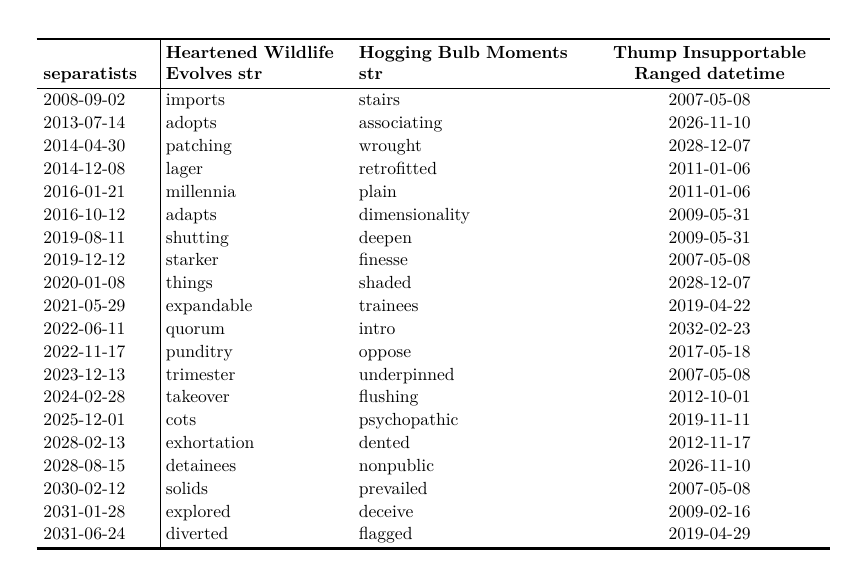
\begin{tikzpicture}[
    auto,
    transform shape,
    nosep/.style={inner sep=0},
    table/.style={
        matrix of nodes,
        row sep=0.125em,
        column sep=0.375em,
        nodes in empty cells,
        nodes={rectangle, scale=0.635, text badly ragged},
    row 1/.style={nodes={text=black, anchor=north, inner ysep=0, text height=0, text depth=0}},
    row 2/.style={nodes={text=black, anchor=south, inner ysep=.2em, minimum height=1.3em, font=\bfseries}},
    column  1/.style={nodes={align=left  }, text height=0.9em, text depth=0.2em, inner xsep=0.375em, inner ysep=0, text width=6.00em},
    column  2/.style={nodes={align=left  }, nosep, text width=10.39em},
    column  3/.style={nodes={align=left  }, nosep, text width=13.23em},
    column  4/.style={nodes={align=center}, nosep, text width=12.28em},
    column  5/.style={text height=0.9em, text depth=0.2em, nosep, text width=0em}   }]
\matrix (TP2KAIMSUSU4U) [table, ampersand replacement=\&]{
            \&             \&                \&            \& \\
 separatists\grtspacer \& Heartened Wildlife Evolves str\grtspacer \& Hogging Bulb Moments str\grtspacer \& Thump Insupportable Ranged datetime\grtspacer \& \\
 2008-09-02 \& imports     \& stairs         \& 2007-05-08 \& \\
 2013-07-14 \& adopts      \& associating    \& 2026-11-10 \& \\
 2014-04-30 \& patching    \& wrought        \& 2028-12-07 \& \\
 2014-12-08 \& lager       \& retrofitted    \& 2011-01-06 \& \\
 2016-01-21 \& millennia   \& plain          \& 2011-01-06 \& \\
 2016-10-12 \& adapts      \& dimensionality \& 2009-05-31 \& \\
 2019-08-11 \& shutting    \& deepen         \& 2009-05-31 \& \\
 2019-12-12 \& starker     \& finesse        \& 2007-05-08 \& \\
 2020-01-08 \& things      \& shaded         \& 2028-12-07 \& \\
 2021-05-29 \& expandable  \& trainees       \& 2019-04-22 \& \\
 2022-06-11 \& quorum      \& intro          \& 2032-02-23 \& \\
 2022-11-17 \& punditry    \& oppose         \& 2017-05-18 \& \\
 2023-12-13 \& trimester   \& underpinned    \& 2007-05-08 \& \\
 2024-02-28 \& takeover    \& flushing       \& 2012-10-01 \& \\
 2025-12-01 \& cots        \& psychopathic   \& 2019-11-11 \& \\
 2028-02-13 \& exhortation \& dented         \& 2012-11-17 \& \\
 2028-08-15 \& detainees   \& nonpublic      \& 2026-11-10 \& \\
 2030-02-12 \& solids      \& prevailed      \& 2007-05-08 \& \\
 2031-01-28 \& explored    \& deceive        \& 2009-02-16 \& \\
 2031-06-24 \& diverted    \& flagged        \& 2019-04-29 \& \\
};

\path[draw, thick] (TP2KAIMSUSU4U-1-1.south west)  -- (TP2KAIMSUSU4U-1-5.south east);
\path[draw, semithick] ([yshift=-0.0625em]TP2KAIMSUSU4U-2-1.south west)  -- ([yshift=-0.0625em]TP2KAIMSUSU4U-2-5.south east);
\path[draw, thick] ([yshift=-0.3125em]TP2KAIMSUSU4U-22-1.base west)  -- ([yshift=-0.3125em]TP2KAIMSUSU4U-22-5.base east);
\path[draw, very thin] ([xshift=-0.1875em]TP2KAIMSUSU4U-1-2.south west)  -- ([yshift=-0.3125em, xshift=-0.1875em]TP2KAIMSUSU4U-22-2.base west);



\end{tikzpicture}

\end{table}%

Comments go here.

\subsection{Test Table: multiindex}\label{test-table-multiindex}

\begin{Shaded}
\begin{Highlighting}[]
\NormalTok{hrw }\OperatorTok{=}\NormalTok{ (}\FloatTok{1.5}\NormalTok{, }\FloatTok{1.0}\NormalTok{, }\FloatTok{0.5}\NormalTok{)}
\NormalTok{sGT(ans[}\StringTok{\textquotesingle{}multiindex\textquotesingle{}}\NormalTok{], }\StringTok{"Multiindex"}\NormalTok{, ratio\_cols}\OperatorTok{=}\StringTok{\textquotesingle{}z\textquotesingle{}}\NormalTok{, aligners}\OperatorTok{=}\NormalTok{\{}\StringTok{\textquotesingle{}w\textquotesingle{}}\NormalTok{: }\StringTok{\textquotesingle{}l\textquotesingle{}}\NormalTok{\},}
\NormalTok{        hrule\_widths}\OperatorTok{=}\NormalTok{hrw)}
\end{Highlighting}
\end{Shaded}

\begin{table}

\caption{\label{tbl-greater-tables-test-2}Output for test table
multiindex}

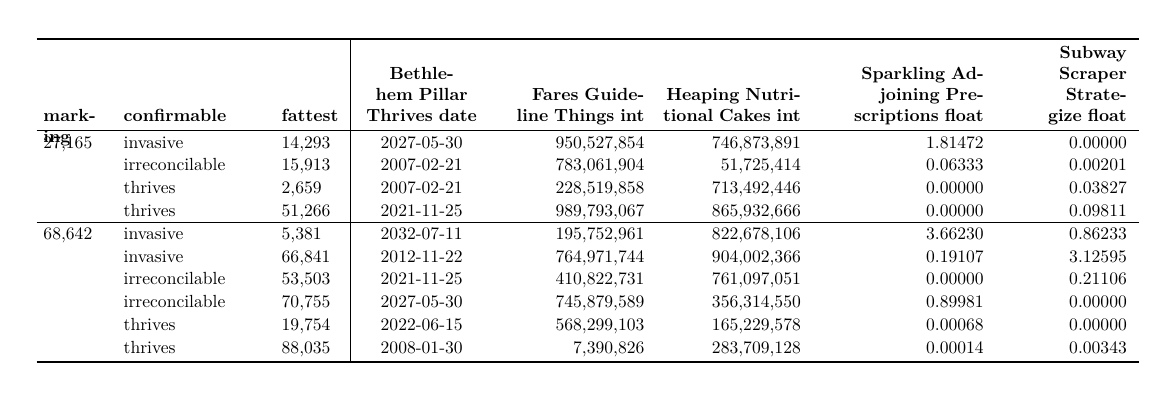
\begin{tikzpicture}[
    auto,
    transform shape,
    nosep/.style={inner sep=0},
    table/.style={
        matrix of nodes,
        row sep=0.125em,
        column sep=0.375em,
        nodes in empty cells,
        nodes={rectangle, scale=0.635, text badly ragged},
    row 1/.style={nodes={text=black, anchor=north, inner ysep=0, text height=0, text depth=0}},
    row 2/.style={nodes={text=black, anchor=south, inner ysep=.2em, minimum height=1.3em, font=\bfseries}},
    column  1/.style={nodes={align=left  }, text height=0.9em, text depth=0.2em, inner xsep=0.375em, inner ysep=0, text width=3.60em},
    column  2/.style={nodes={align=left  }, nosep, text width=8.40em},
    column  3/.style={nodes={align=left  }, nosep, text width=3.60em},
    column  4/.style={nodes={align=center}, nosep, text width=7.55em},
    column  5/.style={nodes={align=right }, nosep, text width=8.31em},
    column  6/.style={nodes={align=right }, nosep, text width=8.31em},
    column  7/.style={nodes={align=right }, nosep, text width=9.82em},
    column  8/.style={nodes={align=right }, nosep, text width=7.55em},
    column  9/.style={text height=0.9em, text depth=0.2em, nosep, text width=0em}   }]
\matrix (TU24XXGXPW72F) [table, ampersand replacement=\&]{
        \&                \&        \&            \&             \&             \&         \&         \& \\
 marking\grtspacer \& confirmable\grtspacer \& fattest\grtspacer \& Bethlehem Pillar Thrives date\grtspacer \& Fares Guideline Things int\grtspacer \& Heaping Nutritional Cakes int\grtspacer \& Sparkling Adjoining Prescriptions float\grtspacer \& Subway Scraper Strategize float\grtspacer \& \\
 27,165 \& invasive       \& 14,293 \& 2027-05-30 \& 950,527,854 \& 746,873,891 \& 1.81472 \& 0.00000 \& \\
        \& irreconcilable \& 15,913 \& 2007-02-21 \& 783,061,904 \&  51,725,414 \& 0.06333 \& 0.00201 \& \\
        \& thrives        \& 2,659  \& 2007-02-21 \& 228,519,858 \& 713,492,446 \& 0.00000 \& 0.03827 \& \\
        \& thrives        \& 51,266 \& 2021-11-25 \& 989,793,067 \& 865,932,666 \& 0.00000 \& 0.09811 \& \\
 68,642 \& invasive       \& 5,381  \& 2032-07-11 \& 195,752,961 \& 822,678,106 \& 3.66230 \& 0.86233 \& \\
        \& invasive       \& 66,841 \& 2012-11-22 \& 764,971,744 \& 904,002,366 \& 0.19107 \& 3.12595 \& \\
        \& irreconcilable \& 53,503 \& 2021-11-25 \& 410,822,731 \& 761,097,051 \& 0.00000 \& 0.21106 \& \\
        \& irreconcilable \& 70,755 \& 2027-05-30 \& 745,879,589 \& 356,314,550 \& 0.89981 \& 0.00000 \& \\
        \& thrives        \& 19,754 \& 2022-06-15 \& 568,299,103 \& 165,229,578 \& 0.00068 \& 0.00000 \& \\
        \& thrives        \& 88,035 \& 2008-01-30 \&   7,390,826 \& 283,709,128 \& 0.00014 \& 0.00343 \& \\
};

\path[draw, thick] (TU24XXGXPW72F-1-1.south west)  -- (TU24XXGXPW72F-1-9.south east);
\path[draw, semithick] ([yshift=-0.0625em]TU24XXGXPW72F-2-1.south west)  -- ([yshift=-0.0625em]TU24XXGXPW72F-2-9.south east);
\path[draw, very thin] ([yshift=-0.0625em]TU24XXGXPW72F-6-1.south west)  -- ([yshift=-0.0625em]TU24XXGXPW72F-6-9.south east);
\path[draw, thick] ([yshift=-0.3125em]TU24XXGXPW72F-12-1.base west)  -- ([yshift=-0.3125em]TU24XXGXPW72F-12-9.base east);
\path[draw, very thin] ([xshift=-0.1875em]TU24XXGXPW72F-1-4.south west)  -- ([yshift=-0.3125em, xshift=-0.1875em]TU24XXGXPW72F-12-4.base west);



\end{tikzpicture}

\end{table}%

Comments go here.

\subsection{Test Table: multicolumns}\label{test-table-multicolumns}

\begin{Shaded}
\begin{Highlighting}[]
\NormalTok{hrw }\OperatorTok{=}\NormalTok{ (}\DecValTok{0}\NormalTok{, }\DecValTok{0}\NormalTok{, }\DecValTok{0}\NormalTok{)}
\NormalTok{sGT(ans[}\StringTok{\textquotesingle{}multicolumns\textquotesingle{}}\NormalTok{], }\StringTok{"Multicolumns"}\NormalTok{, ratio\_cols}\OperatorTok{=}\StringTok{\textquotesingle{}z\textquotesingle{}}\NormalTok{, aligners}\OperatorTok{=}\NormalTok{\{}\StringTok{\textquotesingle{}w\textquotesingle{}}\NormalTok{: }\StringTok{\textquotesingle{}l\textquotesingle{}}\NormalTok{\},}
\NormalTok{        hrule\_widths}\OperatorTok{=}\NormalTok{hrw)}
\end{Highlighting}
\end{Shaded}

\begin{table}

\caption{\label{tbl-greater-tables-test-3}Output for test table
multicolumns}

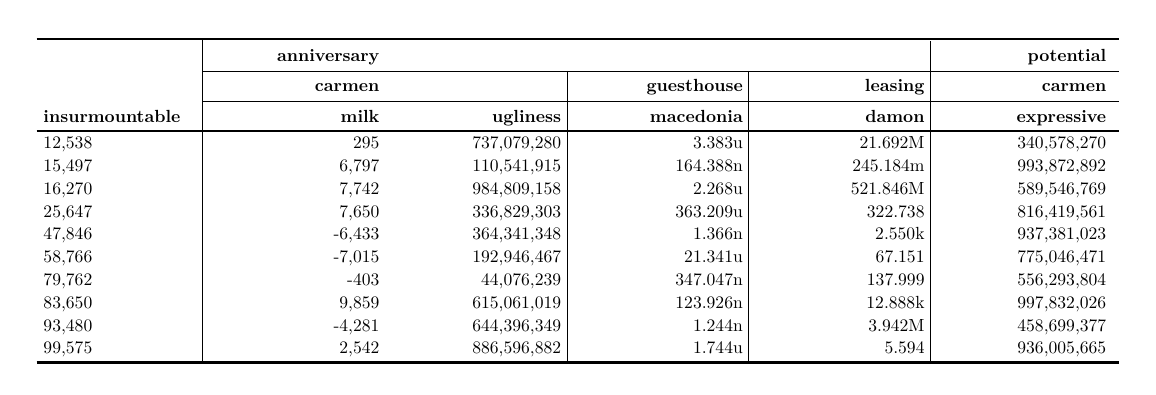
\begin{tikzpicture}[
    auto,
    transform shape,
    nosep/.style={inner sep=0},
    table/.style={
        matrix of nodes,
        row sep=0.125em,
        column sep=0.375em,
        nodes in empty cells,
        nodes={rectangle, scale=0.635, text badly ragged},
    row 1/.style={nodes={text=black, anchor=north, inner ysep=0, text height=0, text depth=0}},
    row 2/.style={nodes={text=black, anchor=south, inner ysep=.2em, minimum height=1.3em, font=\bfseries}},
    row 3/.style={nodes={text=black, anchor=south, inner ysep=.2em, minimum height=1.3em, font=\bfseries}},
    row 4/.style={nodes={text=black, anchor=south, inner ysep=.2em, minimum height=1.3em, font=\bfseries}},
    column  1/.style={nodes={align=left  }, text height=0.9em, text depth=0.2em, inner xsep=0.375em, inner ysep=0, text width=8.40em},
    column  2/.style={nodes={align=right }, nosep, text width=9.75em},
    column  3/.style={nodes={align=right }, nosep, text width=9.75em},
    column  4/.style={nodes={align=right }, nosep, text width=9.75em},
    column  5/.style={nodes={align=right }, nosep, text width=9.75em},
    column  6/.style={nodes={align=right }, nosep, text width=9.75em},
    column  7/.style={text height=0.9em, text depth=0.2em, nosep, text width=0em}   }]
\matrix (TT4ODL4YOAVBP) [table, ampersand replacement=\&]{
        \&        \&             \&           \&           \&             \& \\
 \grtspacer \& anniversary\grtspacer \&  \grtspacer \& \grtspacer \& \grtspacer \& potential\grtspacer \& \\
 \grtspacer \& carmen\grtspacer \&  \grtspacer \& guesthouse\grtspacer \& leasing\grtspacer \& carmen\grtspacer \& \\
 insurmountable\grtspacer \& milk\grtspacer \& ugliness\grtspacer \& macedonia\grtspacer \& damon\grtspacer \& expressive\grtspacer \& \\
 12,538 \&    295 \& 737,079,280 \&    3.383u \&   21.692M \& 340,578,270 \& \\
 15,497 \&  6,797 \& 110,541,915 \&  164.388n \&  245.184m \& 993,872,892 \& \\
 16,270 \&  7,742 \& 984,809,158 \&    2.268u \&  521.846M \& 589,546,769 \& \\
 25,647 \&  7,650 \& 336,829,303 \&  363.209u \&   322.738 \& 816,419,561 \& \\
 47,846 \& -6,433 \& 364,341,348 \&    1.366n \&    2.550k \& 937,381,023 \& \\
 58,766 \& -7,015 \& 192,946,467 \&   21.341u \&    67.151 \& 775,046,471 \& \\
 79,762 \&   -403 \&  44,076,239 \&  347.047n \&   137.999 \& 556,293,804 \& \\
 83,650 \&  9,859 \& 615,061,019 \&  123.926n \&   12.888k \& 997,832,026 \& \\
 93,480 \& -4,281 \& 644,396,349 \&    1.244n \&    3.942M \& 458,699,377 \& \\
 99,575 \&  2,542 \& 886,596,882 \&    1.744u \&     5.594 \& 936,005,665 \& \\
};

\path[draw, thick] (TT4ODL4YOAVBP-1-1.south west)  -- (TT4ODL4YOAVBP-1-7.south east);
\path[draw, semithick] ([yshift=-0.0625em]TT4ODL4YOAVBP-4-1.south west)  -- ([yshift=-0.0625em]TT4ODL4YOAVBP-4-7.south east);
\path[draw, thick] ([yshift=-0.3125em]TT4ODL4YOAVBP-14-1.base west)  -- ([yshift=-0.3125em]TT4ODL4YOAVBP-14-7.base east);
\path[draw, very thin] ([xshift=-0.1875em, yshift=-0.0625em]TT4ODL4YOAVBP-2-2.south west)  -- ([yshift=-0.0625em]TT4ODL4YOAVBP-2-7.south east);
\path[draw, very thin] ([xshift=-0.1875em, yshift=-0.0625em]TT4ODL4YOAVBP-3-2.south west)  -- ([yshift=-0.0625em]TT4ODL4YOAVBP-3-7.south east);
\path[draw, very thin] ([xshift=-0.1875em]TT4ODL4YOAVBP-1-2.south west)  -- ([yshift=-0.3125em, xshift=-0.1875em]TT4ODL4YOAVBP-14-2.base west);
\path[draw, ultra thin] ([xshift=0.1875em, yshift=-0.0625em]TT4ODL4YOAVBP-1-5.south east)  -- ([yshift=-0.3125em, xshift=0.1875em]TT4ODL4YOAVBP-14-5.base east);
\path[draw, ultra thin] ([xshift=0.1875em, yshift=-0.0625em]TT4ODL4YOAVBP-2-3.south east)  -- ([yshift=-0.3125em, xshift=0.1875em]TT4ODL4YOAVBP-14-3.base east);
\path[draw, ultra thin] ([xshift=0.1875em, yshift=-0.0625em]TT4ODL4YOAVBP-2-4.south east)  -- ([yshift=-0.3125em, xshift=0.1875em]TT4ODL4YOAVBP-14-4.base east);



\end{tikzpicture}

\end{table}%

Comments go here.

\subsection{Test Table: complex}\label{test-table-complex}

\begin{Shaded}
\begin{Highlighting}[]
\NormalTok{hrw }\OperatorTok{=}\NormalTok{ (}\FloatTok{1.5}\NormalTok{, }\FloatTok{1.0}\NormalTok{, }\FloatTok{0.5}\NormalTok{)}
\NormalTok{sGT(ans[}\StringTok{\textquotesingle{}complex\textquotesingle{}}\NormalTok{], }\StringTok{"Complex"}\NormalTok{, ratio\_cols}\OperatorTok{=}\StringTok{\textquotesingle{}z\textquotesingle{}}\NormalTok{, aligners}\OperatorTok{=}\NormalTok{\{}\StringTok{\textquotesingle{}w\textquotesingle{}}\NormalTok{: }\StringTok{\textquotesingle{}l\textquotesingle{}}\NormalTok{\},}
\NormalTok{        hrule\_widths}\OperatorTok{=}\NormalTok{hrw)}
\end{Highlighting}
\end{Shaded}

\begin{table}

\caption{\label{tbl-greater-tables-test-4}Output for test table complex}

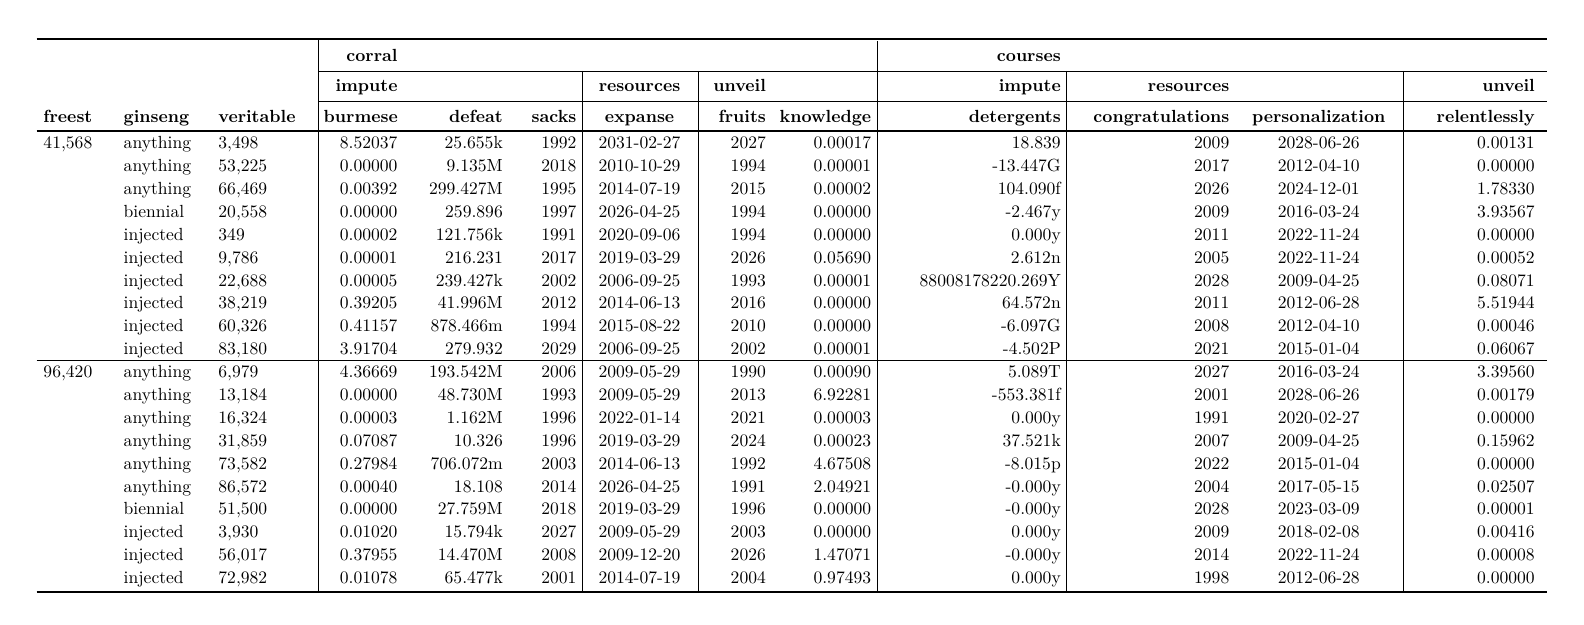
\begin{tikzpicture}[
    auto,
    transform shape,
    nosep/.style={inner sep=0},
    table/.style={
        matrix of nodes,
        row sep=0.125em,
        column sep=0.375em,
        nodes in empty cells,
        nodes={rectangle, scale=0.635, text badly ragged},
    row 1/.style={nodes={text=black, anchor=north, inner ysep=0, text height=0, text depth=0}},
    row 2/.style={nodes={text=black, anchor=south, inner ysep=.2em, minimum height=1.3em, font=\bfseries}},
    row 3/.style={nodes={text=black, anchor=south, inner ysep=.2em, minimum height=1.3em, font=\bfseries}},
    row 4/.style={nodes={text=black, anchor=south, inner ysep=.2em, minimum height=1.3em, font=\bfseries}},
    column  1/.style={nodes={align=left  }, text height=0.9em, text depth=0.2em, inner xsep=0.375em, inner ysep=0, text width=3.60em},
    column  2/.style={nodes={align=left  }, nosep, text width=4.80em},
    column  3/.style={nodes={align=left  }, nosep, text width=5.40em},
    column  4/.style={nodes={align=right }, nosep, text width=4.20em},
    column  5/.style={nodes={align=right }, nosep, text width=5.40em},
    column  6/.style={nodes={align=right }, nosep, text width=3.60em},
    column  7/.style={nodes={align=center}, nosep, text width=6.00em},
    column  8/.style={nodes={align=right }, nosep, text width=3.60em},
    column  9/.style={nodes={align=right }, nosep, text width=5.40em},
    column 10/.style={nodes={align=right }, nosep, text width=10.20em},
    column 11/.style={nodes={align=right }, nosep, text width=9.00em},
    column 12/.style={nodes={align=center}, nosep, text width=9.00em},
    column 13/.style={nodes={align=right }, nosep, text width=7.20em},
    column 14/.style={text height=0.9em, text depth=0.2em, nosep, text width=0em}   }]
\matrix (T5VJIEBLSIK73) [table, ampersand replacement=\&]{
        \&          \&        \&         \&           \&      \&            \&      \&         \&                   \&      \&            \&         \& \\
 \grtspacer \& \grtspacer \& \grtspacer \& corral\grtspacer \& \grtspacer \& \grtspacer \& \grtspacer \& \grtspacer \& \grtspacer \& courses\grtspacer \& \grtspacer \& \grtspacer \& \grtspacer \& \\
 \grtspacer \& \grtspacer \& \grtspacer \& impute\grtspacer \& \grtspacer \& \grtspacer \& resources\grtspacer \& unveil\grtspacer \& \grtspacer \&  impute\grtspacer \& resources\grtspacer \& \grtspacer \& unveil\grtspacer \& \\
 freest\grtspacer \& ginseng\grtspacer \& veritable\grtspacer \& burmese\grtspacer \& defeat\grtspacer \& sacks\grtspacer \& expanse\grtspacer \& fruits\grtspacer \& knowledge\grtspacer \& detergents\grtspacer \& congratulations\grtspacer \& personalization\grtspacer \& relentlessly\grtspacer \& \\
 41,568 \& anything \& 3,498  \& 8.52037 \&   25.655k \& 1992 \& 2031-02-27 \& 2027 \& 0.00017 \&            18.839 \& 2009 \& 2028-06-26 \& 0.00131 \& \\
        \& anything \& 53,225 \& 0.00000 \&    9.135M \& 2018 \& 2010-10-29 \& 1994 \& 0.00001 \&          -13.447G \& 2017 \& 2012-04-10 \& 0.00000 \& \\
        \& anything \& 66,469 \& 0.00392 \&  299.427M \& 1995 \& 2014-07-19 \& 2015 \& 0.00002 \&          104.090f \& 2026 \& 2024-12-01 \& 1.78330 \& \\
        \& biennial \& 20,558 \& 0.00000 \&   259.896 \& 1997 \& 2026-04-25 \& 1994 \& 0.00000 \&           -2.467y \& 2009 \& 2016-03-24 \& 3.93567 \& \\
        \& injected \& 349    \& 0.00002 \&  121.756k \& 1991 \& 2020-09-06 \& 1994 \& 0.00000 \&            0.000y \& 2011 \& 2022-11-24 \& 0.00000 \& \\
        \& injected \& 9,786  \& 0.00001 \&   216.231 \& 2017 \& 2019-03-29 \& 2026 \& 0.05690 \&            2.612n \& 2005 \& 2022-11-24 \& 0.00052 \& \\
        \& injected \& 22,688 \& 0.00005 \&  239.427k \& 2002 \& 2006-09-25 \& 1993 \& 0.00001 \&  88008178220.269Y \& 2028 \& 2009-04-25 \& 0.08071 \& \\
        \& injected \& 38,219 \& 0.39205 \&   41.996M \& 2012 \& 2014-06-13 \& 2016 \& 0.00000 \&           64.572n \& 2011 \& 2012-06-28 \& 5.51944 \& \\
        \& injected \& 60,326 \& 0.41157 \&  878.466m \& 1994 \& 2015-08-22 \& 2010 \& 0.00000 \&           -6.097G \& 2008 \& 2012-04-10 \& 0.00046 \& \\
        \& injected \& 83,180 \& 3.91704 \&   279.932 \& 2029 \& 2006-09-25 \& 2002 \& 0.00001 \&           -4.502P \& 2021 \& 2015-01-04 \& 0.06067 \& \\
 96,420 \& anything \& 6,979  \& 4.36669 \&  193.542M \& 2006 \& 2009-05-29 \& 1990 \& 0.00090 \&            5.089T \& 2027 \& 2016-03-24 \& 3.39560 \& \\
        \& anything \& 13,184 \& 0.00000 \&   48.730M \& 1993 \& 2009-05-29 \& 2013 \& 6.92281 \&         -553.381f \& 2001 \& 2028-06-26 \& 0.00179 \& \\
        \& anything \& 16,324 \& 0.00003 \&    1.162M \& 1996 \& 2022-01-14 \& 2021 \& 0.00003 \&            0.000y \& 1991 \& 2020-02-27 \& 0.00000 \& \\
        \& anything \& 31,859 \& 0.07087 \&    10.326 \& 1996 \& 2019-03-29 \& 2024 \& 0.00023 \&           37.521k \& 2007 \& 2009-04-25 \& 0.15962 \& \\
        \& anything \& 73,582 \& 0.27984 \&  706.072m \& 2003 \& 2014-06-13 \& 1992 \& 4.67508 \&           -8.015p \& 2022 \& 2015-01-04 \& 0.00000 \& \\
        \& anything \& 86,572 \& 0.00040 \&    18.108 \& 2014 \& 2026-04-25 \& 1991 \& 2.04921 \&           -0.000y \& 2004 \& 2017-05-15 \& 0.02507 \& \\
        \& biennial \& 51,500 \& 0.00000 \&   27.759M \& 2018 \& 2019-03-29 \& 1996 \& 0.00000 \&           -0.000y \& 2028 \& 2023-03-09 \& 0.00001 \& \\
        \& injected \& 3,930  \& 0.01020 \&   15.794k \& 2027 \& 2009-05-29 \& 2003 \& 0.00000 \&            0.000y \& 2009 \& 2018-02-08 \& 0.00416 \& \\
        \& injected \& 56,017 \& 0.37955 \&   14.470M \& 2008 \& 2009-12-20 \& 2026 \& 1.47071 \&           -0.000y \& 2014 \& 2022-11-24 \& 0.00008 \& \\
        \& injected \& 72,982 \& 0.01078 \&   65.477k \& 2001 \& 2014-07-19 \& 2004 \& 0.97493 \&            0.000y \& 1998 \& 2012-06-28 \& 0.00000 \& \\
};

\path[draw, thick] (T5VJIEBLSIK73-1-1.south west)  -- (T5VJIEBLSIK73-1-14.south east);
\path[draw, thick] ([yshift=-0.3125em]T5VJIEBLSIK73-24-1.base west)  -- ([yshift=-0.3125em]T5VJIEBLSIK73-24-14.base east);
\path[draw, semithick] ([yshift=-0.0625em]T5VJIEBLSIK73-4-1.south west)  -- ([yshift=-0.0625em]T5VJIEBLSIK73-4-14.south east);
\path[draw, very thin] ([yshift=-0.0625em]T5VJIEBLSIK73-14-1.south west)  -- ([yshift=-0.0625em]T5VJIEBLSIK73-14-14.south east);
\path[draw, very thin] ([xshift=-0.1875em, yshift=-0.0625em]T5VJIEBLSIK73-2-4.south west)  -- ([yshift=-0.0625em]T5VJIEBLSIK73-2-14.south east);
\path[draw, very thin] ([xshift=-0.1875em, yshift=-0.0625em]T5VJIEBLSIK73-3-4.south west)  -- ([yshift=-0.0625em]T5VJIEBLSIK73-3-14.south east);
\path[draw, very thin] ([xshift=-0.1875em]T5VJIEBLSIK73-1-4.south west)  -- ([yshift=-0.3125em, xshift=-0.1875em]T5VJIEBLSIK73-24-4.base west);
\path[draw, ultra thin] ([xshift=0.1875em, yshift=-0.0625em]T5VJIEBLSIK73-1-9.south east)  -- ([yshift=-0.3125em, xshift=0.1875em]T5VJIEBLSIK73-24-9.base east);
\path[draw, ultra thin] ([xshift=0.1875em, yshift=-0.0625em]T5VJIEBLSIK73-2-6.south east)  -- ([yshift=-0.3125em, xshift=0.1875em]T5VJIEBLSIK73-24-6.base east);
\path[draw, ultra thin] ([xshift=0.1875em, yshift=-0.0625em]T5VJIEBLSIK73-2-7.south east)  -- ([yshift=-0.3125em, xshift=0.1875em]T5VJIEBLSIK73-24-7.base east);
\path[draw, ultra thin] ([xshift=0.1875em, yshift=-0.0625em]T5VJIEBLSIK73-2-10.south east)  -- ([yshift=-0.3125em, xshift=0.1875em]T5VJIEBLSIK73-24-10.base east);
\path[draw, ultra thin] ([xshift=0.1875em, yshift=-0.0625em]T5VJIEBLSIK73-2-12.south east)  -- ([yshift=-0.3125em, xshift=0.1875em]T5VJIEBLSIK73-24-12.base east);



\end{tikzpicture}

\end{table}%

Comments go here.




\end{document}
